% ----------------------------------------------------------------------
%                             Preamble
% ----------------------------------------------------------------------

\documentclass[xcolor=svgnames,aspectratio=32,8pt]{beamer}
% \usepackage[size=custom,width=20.3646752982,height=14.4]{beamerposter}

\usepackage[utf8]    {inputenc}
\usepackage[T1]      {fontenc}
\usepackage[english] {babel}

\usepackage{amsmath,amsfonts,graphicx,pgfplots}
\usepackage{beamerleanprogress}
\usepackage{caption}
\usepackage{textcomp}

% \usepackage{handoutWithNotes}

% \pgfpagesuselayout{2 on 1 with notes landscape}[a4paper,border shrink=5mm]

\usebackgroundtemplate{%
  
\includegraphics[width=\paperwidth,height=\paperheight]{BG/Title32.png}}


\title
  [Optimal Configuration of Distribution Networks under Technical Constraints based on Predictive Methods]
  {Optimal Configuration of Distribution Networks under Technical Constraints based on Predictive Methods}

\author
  [B. P. Swaminathan]
  {Master's Thesis Dissertation by\\Bhargav P Swaminathan\\{\small M2 - Smart Grids and Buildings}}

\date
  {June 25, 2014}

\institute
  {Supervisors:\\Rapha\"{e}l Caire \& Vincent Debusschere}


\begin{document}

% ----------------------------------------------------------------------
% For Align Environment

\setlength{\abovedisplayskip}{0pt}
\setlength{\belowdisplayskip}{0pt}
\setlength{\abovedisplayshortskip}{0pt}
\setlength{\belowdisplayshortskip}{0pt}

% ----------------------------------------------------------------------

\setbeamertemplate{title page}[default][left]
\maketitle

\usebackgroundtemplate{%
  
\includegraphics[width=\paperwidth,height=\paperheight]{BG/Slides32.png}}

% ----------------------------------------------------------------------
%                             Introduction
% ----------------------------------------------------------------------

\section
  {Introduction}

\begin{frame}
  {Agenda}{for today's presentation}
  % \begin{itemize}
  % \item Background
  % \item Introduction to the Problem
  % \item Literature Review\pause
  % \item Definition of Requirements
  % \item Test Networks and Models
  % \item The Algorithm\pause
  % \item Results Obtained
  % \item Conclusions and Perspectives
  % \item Future Work
  % \end{itemize}

  \begin{minipage}[!h]{0.5\textwidth}
    \begin{block}{Introduction}
    \begin{itemize}
    \item Background
    \item Introduction to the Problem
    \item Literature Review
    \end{itemize}
    \end{block}
  \pause
  \end{minipage}%
  \begin{minipage}[!h]{0.5\textwidth}
    \begin{block}{Preliminary Work}
    \begin{itemize}
    \item Work Objectives
    \item Test Networks
    \item Day-ahead Load and DRES Models
    \end{itemize}
    \end{block}
  \pause
  \end{minipage}

  \begin{minipage}[!h]{0.5\textwidth}
    \begin{alertblock}{The Algorithm}
    \begin{itemize}
    \item Formulation \& Economic Models
    \item Components
    \item Working of the Algorithm
    \end{itemize}
    \end{alertblock}
  \pause
  \end{minipage}%
  \begin{minipage}[!h]{0.5\textwidth}
    \begin{exampleblock}{Results \& Conclusions}
    \begin{itemize}
    \item Results Obtained
    \item Conclusions
    \item Future Work
    \end{itemize}
    \end{exampleblock}
  \end{minipage}

\end{frame}

% ----------------------------------------------------------------------

\begin{frame}
  {Background}{Electrical Distribution Network Optimization}

  \begin{itemize}
    \item \textbf{Merlin and Back} method, close to 40 years ago! \pause
    \vspace{0.2cm}
    \item Developments in Optimization. \pause
    \vspace{0.2cm}
    \item Shift from \textbf{single-objective} to \textbf{multiple-objectives}, to genetic, and other nature-inspired methods. \pause
    \vspace{0.2cm}
    \item Problems with DRES integration! \pause
    \vspace{0.2cm}
    \item Distribution network optimization has to take a new, giant leap. \pause
    \vspace{0.2cm}
    \item This work proposes a method to take this leap!
  \end{itemize}

\end{frame}

% ----------------------------------------------------------------------

\begin{frame}
  {Introduction}{to the problem}

  Why is large-scale DRES integration is a problem?

  \begin{itemize}
    \item Variability / Intermittency
    \item Bi-directional Power Flows
    \item Grid Weakening
    \item Network Imbalance
    \item Fault Current Issues
    \item And finally: Money!
  \end{itemize}

  \vspace{0.4cm}
  There is a \textbf{real need} to find solutions that assuage the problem with the integration of DRES.

  % \begin{minipage}[!h]{0.3\paperwidth}
  % \centering
  % 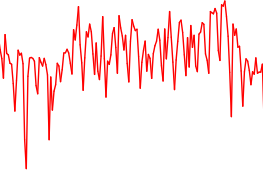
\includegraphics[width=0.3\paperwidth]{OtherImages/Intermittency.png}\\
  % Intermittency
  % \end{minipage}%
  % \begin{minipage}[!h]{0.3\paperwidth}
  % \centering
  % 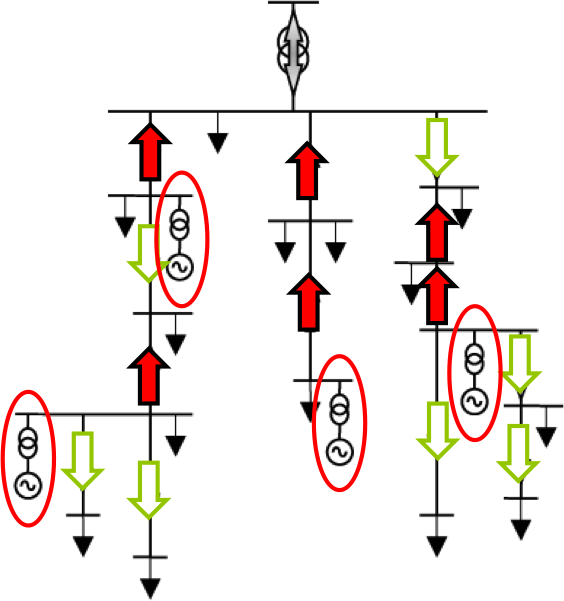
\includegraphics[width=0.3\paperwidth]{OtherImages/ODbg.png}\\
  % Bi-directional Power Flows
  % \end{minipage}%
  % \begin{minipage}[!h]{0.3\paperwidth}
  % \centering
  % % 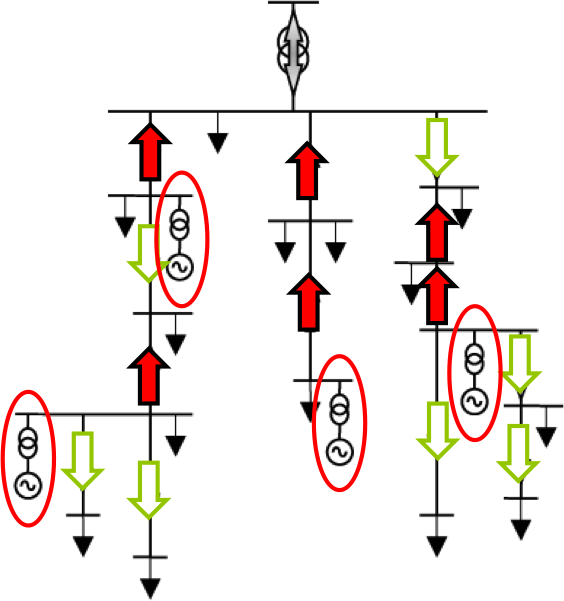
\includegraphics[width=0.3\paperwidth]{OtherImages/ODbg.png}
  % % Bi-directional Power Flows
  % \end{minipage}%
\end{frame}

% ----------------------------------------------------------------------

\begin{frame}
  {Literature Review}{Current Work in the Domain}

  \textbf{Forecasting:}
  \begin{itemize}
    \item A lot of work has been done in forecasting for DRES and Loads
    \item Persistency / NWP based methods
    \item Both traditional and stochastic load forecasting: fairly \textbf{mature}
    \item But are they applicable to Distribution Networks?
  \end{itemize}\pause
  \vspace{0.5cm}
  \textbf{Distribution Network Optimization:}
  \begin{itemize}
    \item ``Snapshot'' based optimization
    \item Few instances of multi-temporal optimization
    \item Even they don't take a lot of issues into account
    \item Hence, there is a real need for a novel tool
  \end{itemize}

\end{frame}

% ----------------------------------------------------------------------
%                             Preparation
% ----------------------------------------------------------------------

\section
  {Preliminary Work}

\begin{frame}<handout:0>
  {}{}
  \begin{changemargin}{-1cm}{-1cm}
  \centering
  {\Huge \color{evolvdso} Part II\\\ \\Preliminary Work}
  \end{changemargin}
\end{frame}

\begin{frame}
  {Work Objectives}
  The following requirements were defined for the work to be done. The work should:\\
  \vspace{0.2cm}
  \begin{itemize}
  \item Create a \textbf{day-ahead schedule} based on DRES and Load forecasts \pause
  \vspace{0.2cm}
  \item Effectively utilize all  \textbf{flexibilities} in distribution networks for optimization \pause
  \vspace{0.2cm}
  \item \textbf{NOT only use ``snapshot''} based optimziation, i.e. should be multi-temporal \pause
  \vspace{0.2cm}
  \item Be \textbf{multi-objective} \pause
  \vspace{0.2cm}
  \item Be \textbf{modular} \pause
  \vspace{0.2cm}
  \item Be a \textbf{black box} for end-users
  \end{itemize}
\end{frame}

% ----------------------------------------------------------------------

\begin{frame}
{Test Networks}{Network 1 - PREDIS Urban Network}

  \vspace{0.5cm}
  \begin{changemargin}{-0.8cm}{-1cm}

    \begin{minipage}[!h]{0.55\paperwidth}

      \centering
      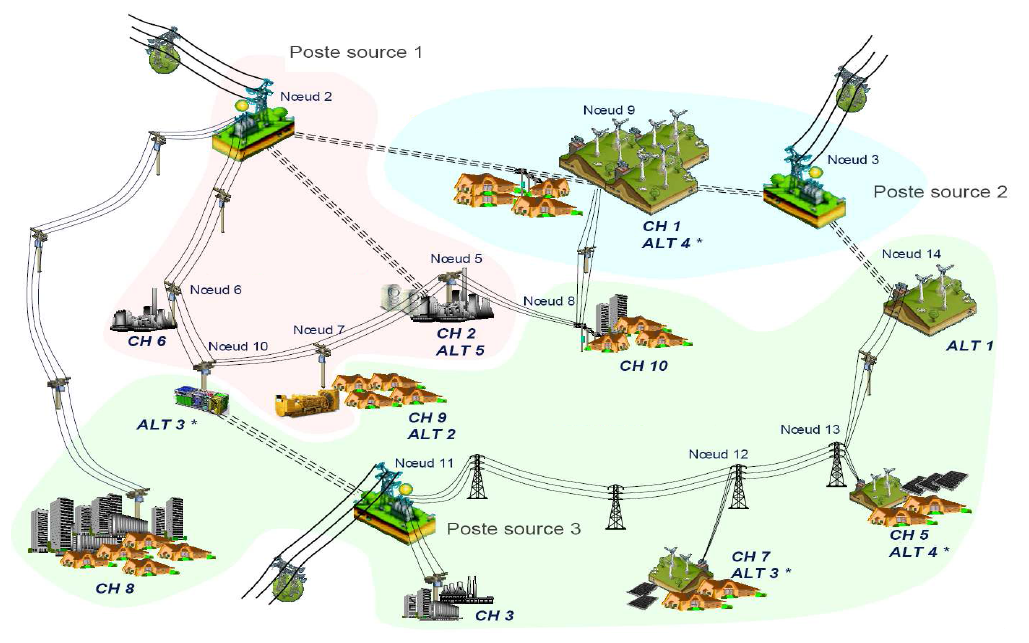
\includegraphics[width=0.55\paperwidth]{NwImages/PredisG.png}

    \end{minipage}%
    \begin{minipage}[!h]{0.45\paperwidth}
      % \begin{minipage}[!h]{0.25\paperwidth}
      % \centering
      % \adjustbox{max width=0.2\paperwidth}{
      % \begin{tabular}{cc}
      % \rowcolor{gray!25}
      % \multicolumn{2}{c}{Base Values}\\
      % \hline
      % Voltage & $11$ kV\\
      % % \hline
      % \rowcolor{gray!15}
      % Power & $100$ MVA\\
      % % \hline
      % Current &  $5248.6$ A\\
      % % \hline
      % \rowcolor{gray!15}
      % Impedance & $1.21$ $\Omega$\\
      % \hline
      % \end{tabular}
      % }
      % \end{minipage}%
      % \begin{minipage}[!h]{0.25\paperwidth}
      % \centering
      % \adjustbox{max width=0.2\paperwidth}{

      % \begin{tabular}{cc}
      % % \hline
      % \rowcolor{gray!25}
      % \textbf{Lines} & \textbf{I max}\\
      % \hline
      % $7$, $8$, $10$ \& $11$ & $195$ A\\
      % % \hline
      % \rowcolor{gray!15}
      % $14$ & $302$ A\\
      % % \hline
      % $4$, $9$ \& $15-17$ & $363$ A\\
      % % \hline
      % \rowcolor{gray!15}
      % $6$ & $402$ A\\
      % % \hline
      % $5$ & $538$ A\\
      % % \hline
      % \rowcolor{gray!15}
      % $1-3$, $12$ \& $13$ & $1$ pu\\
      % \hline
      % \end{tabular}

      % }
      % \end{minipage}

      % \vspace{0.5cm}

      \begin{itemize}
      \setlength{\itemindent}{-0.5em}

      \item Reduced-scale Urban Network
      \item 14 buses, 17 lines
      \item Connected Load: 26.5 MVA
      \item Installed DRES Capacity: 27 MW
      \item Undervoltage and overcurrent problems

      \end{itemize}

    \end{minipage}

  \end{changemargin}

\end{frame}

% ----------------------------------------------------------------------

\begin{frame}
{Test Networks}{Network 2 - IEEE $11$kV Rural Network}
\begin{changemargin}{-1cm}{-1cm} 

\begin{minipage}[!h]{.5\paperwidth}
\centering
\vspace{0.4cm}
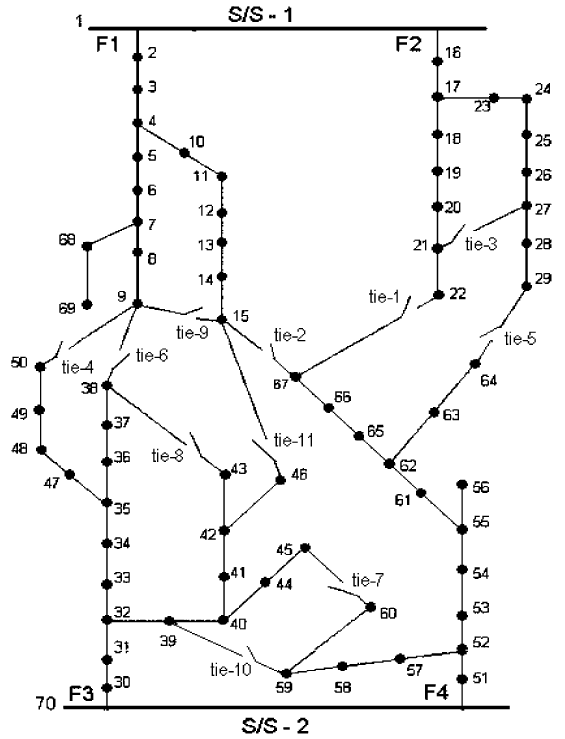
\includegraphics[width=0.35\paperwidth]{NwImages/Rural_Network.png}
\end{minipage}%
% \begin{minipage}[!h]{.3\paperwidth}
% \centering
% % \begin{table}[!h]
% \adjustbox{max width=0.3\paperwidth}{
% \begin{tabular}{cc}
%   \rowcolor{gray!25}
%   \multicolumn{2}{c}{Base Values}\\
%   \hline
%   Voltage & $11$ kV\\
%   % \hline
%   \rowcolor{gray!15}
%   Power & $10$ MVA\\
%   % \hline
%   Current &  $524.86$ A\\
%   % \hline
%   \rowcolor{gray!15}
%   Impedance & $12.1$ $\Omega$\\
%   \hline
%   \end{tabular}
% % \end{table}
% }
% \\\ \\\ \\\
% \adjustbox{max width=0.3\paperwidth}{
% \begin{tabular}{cc}
%   % \hline
%   \rowcolor{gray!25}
%   \textbf{Lines} & \textbf{I max}\\
%   \hline
%   Tie Lines & $234$ A\\
%   % \hline
%   \rowcolor{gray!15}
%   $1-18$, $17-23$ & $270$ A\\
%   $31-39$, $52-57$ & $270$ A \\
%   % \hline
%   \rowcolor{gray!15}
%   $9-16$, $24-30$ & $208$ A\\
%   $40-51$, $58-68$ & $208$ A\\
%   \hline
%   \end{tabular}
% }
% \end{minipage}%
\begin{minipage}[!h]{.5\paperwidth}
\begin{itemize}
% \setlength{\itemindent}{-1em}
\item Larger Network than PREDIS
\item 70 buses, 79 lines
\item Connected Load: 5.41 MVA
\item DRES Info not available
\end{itemize}
\end{minipage}

\end{changemargin}
\end{frame}

% ----------------------------------------------------------------------

\begin{frame}
{Day-ahead Load and DRES Models}{Raw Models}

\begin{changemargin}{-1cm}{-1cm} 
  \vspace{0.5cm}
  \begin{minipage}[!h]{0.4\paperwidth}

  \begin{itemize}
  \item \textbf{Two raw models} extracted from literature.
  \item Specific weights for different types of loads.
  \item Residential, Industrial, Commercial, and Public Lighting.
  \item DRES Models: Values based on characteristic curves.
  \item Variation of Solar Power etc., taken into account.
  \end{itemize}

  \end{minipage}%
  \begin{minipage}[!h]{0.6\paperwidth}

  \begin{figure}[!h]
  \centering
  \newlength\figureheight
  \newlength\figurewidth
  \setlength\figureheight{2cm}
  \setlength\figurewidth{0.5\paperwidth}
  % This file was created by matlab2tikz v0.4.6 running on MATLAB 8.2.
% Copyright (c) 2008--2014, Nico Schlömer <nico.schloemer@gmail.com>
% All rights reserved.
% Minimal pgfplots version: 1.3
% 
% The latest updates can be retrieved from
%   http://www.mathworks.com/matlabcentral/fileexchange/22022-matlab2tikz
% where you can also make suggestions and rate matlab2tikz.
% 
\begin{tikzpicture}

\begin{axis}[%
width=\figurewidth,
height=\figureheight,
scale only axis,
xmin=0,
xmax=23,
xtick={ 0,  2,  4,  6,  8, 10, 12, 14, 16, 18, 20, 22},
xlabel={Time (hour)},
ymin=0,
ymax=1.8,
ylabel={Weights},
axis x line*=bottom,
axis y line*=left,
legend style={draw=black,fill=white,legend cell align=left, at={(0.5,-0.25)},anchor=north, legend columns=2}
]
\addplot [color=red,solid,line width=1.0pt,mark=square,mark options={solid}]
  table[row sep=crcr]{
0	1.2	\\
1	1.05	\\
2	0.85	\\
3	0.95	\\
4	0.9	\\
5	0.8	\\
6	0.8	\\
7	0.6	\\
8	0.65	\\
9	0.55	\\
10	0.6	\\
11	0.65	\\
12	0.7	\\
13	0.75	\\
14	0.75	\\
15	0.75	\\
16	0.8	\\
17	0.85	\\
18	1.35	\\
19	1.6	\\
20	1.65	\\
21	1.65	\\
22	1.7	\\
23	1.55	\\
};
\addlegendentry{Residential};

\addplot [color=green,solid,line width=1.0pt,mark=asterisk,mark options={solid}]
  table[row sep=crcr]{
0	0.9	\\
1	0.85	\\
2	0.85	\\
3	0.85	\\
4	0.8	\\
5	0.8	\\
6	0.8	\\
7	0.8	\\
8	0.9	\\
9	1.15	\\
10	1.15	\\
11	1.2	\\
12	1.15	\\
13	1	\\
14	1.2	\\
15	1.15	\\
16	1.1	\\
17	1.05	\\
18	1	\\
19	1	\\
20	1.05	\\
21	1.05	\\
22	1	\\
23	0.95	\\
};
\addlegendentry{Industrial};

\addplot [color=blue,solid,line width=1.0pt,mark=o,mark options={solid}]
  table[row sep=crcr]{
0	0.5	\\
1	0.5	\\
2	0.45	\\
3	0.45	\\
4	0.4	\\
5	0.4	\\
6	0.5	\\
7	0.55	\\
8	1.15	\\
9	1.5	\\
10	1.55	\\
11	1.55	\\
12	1.6	\\
13	1.45	\\
14	1.5	\\
15	1.5	\\
16	1.5	\\
17	1.45	\\
18	1.3	\\
19	1.15	\\
20	0.85	\\
21	0.75	\\
22	0.6	\\
23	0.6	\\
};
\addlegendentry{Commercial};

\addplot [color=black,solid,line width=1.0pt,mark=x,mark options={solid}]
  table[row sep=crcr]{
0	0.93	\\
1	0.93	\\
2	0.92	\\
3	0.93	\\
4	0.93	\\
5	0.93	\\
6	0.93	\\
7	0.95	\\
8	0.125	\\
9	0.05	\\
10	0.05	\\
11	0.05	\\
12	0.05	\\
13	0.05	\\
14	0.05	\\
15	0.05	\\
16	0.05	\\
17	0.025	\\
18	0.85	\\
19	0.93	\\
20	0.93	\\
21	0.93	\\
22	0.93	\\
23	0.93	\\
};
\addlegendentry{Lighting};

\end{axis}
\end{tikzpicture}%
  \end{figure}
  \begin{figure}[!h]
  \centering
  \setlength\figureheight{2cm}
  \setlength\figurewidth{0.5\paperwidth}
  % This file was created by matlab2tikz v0.4.6 running on MATLAB 8.2.
% Copyright (c) 2008--2014, Nico Schlömer <nico.schloemer@gmail.com>
% All rights reserved.
% Minimal pgfplots version: 1.3
% 
% The latest updates can be retrieved from
%   http://www.mathworks.com/matlabcentral/fileexchange/22022-matlab2tikz
% where you can also make suggestions and rate matlab2tikz.
% 
\begin{tikzpicture}[scale=0.8]

\tikzset{mark size=1.5}
\begin{axis}[%
width=\figurewidth,
height=\figureheight,
scale only axis,
xmin=0,
xmax=23,
xtick={ 0,  2,  4,  6,  8, 10, 12, 14, 16, 18, 20, 22},
xlabel={Time (hour) - Model 2},
x label style={at={(0.5,0.1)},anchor=north},
ymin=0,
ymax=1.1,
ylabel={Weights},
y label style={at={(0.075,0.75)},anchor=east},
axis x line*=bottom,
axis y line*=left,
legend style={draw=black,fill=white,legend cell align=left, at={(0.5,-0.75)},anchor=north, legend columns=2}
]
\addplot [color=red,solid,line width=1.0pt,mark=square,mark options={solid}]
  table[row sep=crcr]{
0	0.37	\\
1	0.35	\\
2	0.3	\\
3	0.27	\\
4	0.27	\\
5	0.25	\\
6	0.25	\\
7	0.25	\\
8	0.23	\\
9	0.2	\\
10	0.75	\\
11	0.82	\\
12	0.7	\\
13	0.925	\\
14	0.725	\\
15	0.4	\\
16	0.7	\\
17	0.8	\\
18	0.925	\\
19	0.98	\\
20	1.025	\\
21	0.8	\\
22	0.575	\\
23	0.4	\\
};
\addlegendentry{Residential};

\addplot [color=green,solid,line width=1.0pt,mark=asterisk,mark options={solid}]
  table[row sep=crcr]{
0	0.5	\\
1	0.375	\\
2	0.29	\\
3	0.275	\\
4	0.275	\\
5	0.23	\\
6	0.23	\\
7	0.42	\\
8	0.4	\\
9	0.58	\\
10	0.57	\\
11	0.52	\\
12	0.5	\\
13	0.475	\\
14	0.6	\\
15	0.5	\\
16	0.675	\\
17	0.6	\\
18	0.875	\\
19	0.9	\\
20	0.95	\\
21	1	\\
22	0.95	\\
23	0.775	\\
};
\addlegendentry{Industrial};

\addplot [color=blue,solid,line width=1.0pt,mark=o,mark options={solid}]
  table[row sep=crcr]{
0	0.275	\\
1	0.275	\\
2	0.275	\\
3	0.275	\\
4	0.275	\\
5	0.3	\\
6	0.35	\\
7	0.75	\\
8	0.88	\\
9	0.95	\\
10	0.925	\\
11	0.95	\\
12	0.925	\\
13	0.9	\\
14	0.88	\\
15	0.8	\\
16	0.6	\\
17	0.5	\\
18	0.45	\\
19	0.41	\\
20	0.4	\\
21	0.42	\\
22	0.41	\\
23	0.35	\\
};
\addlegendentry{Commercial};

\addplot [color=black,solid,line width=1.0pt,mark=x,mark options={solid}]
  table[row sep=crcr]{
0	0.93	\\
1	0.93	\\
2	0.92	\\
3	0.93	\\
4	0.93	\\
5	0.93	\\
6	0.93	\\
7	0.95	\\
8	0.125	\\
9	0.05	\\
10	0.05	\\
11	0.05	\\
12	0.05	\\
13	0.05	\\
14	0.05	\\
15	0.05	\\
16	0.05	\\
17	0.025	\\
18	0.85	\\
19	0.93	\\
20	0.93	\\
21	0.93	\\
22	0.93	\\
23	0.93	\\
};
\addlegendentry{Lighting};

\end{axis}
\end{tikzpicture}%
  \end{figure}

  \end{minipage}

\end{changemargin}
\end{frame}

% ----------------------------------------------------------------------

\begin{frame}
  {Day-ahead Load and DRES Models}{Models Applied to Networks}
  \vspace{0.3cm}
  \begin{changemargin}{-0.9cm}{-0.9cm} 
  \centering
  \begin{minipage}[!h]{0.45\paperwidth}

    \centering
    \begin{alertblock}{Load Model A}
    \begin{itemize}
      \item This model consists of a simple association of each load type to one node.
      \item The load in each node varies accordingly for a given 24 hour period.
    \end{itemize}
    \end{alertblock}

  \end{minipage}%
  \begin{minipage}[!h]{0.45\paperwidth}
    \centering
    \begin{block}{Load Model B}
    Each node has a particular \% of loads of each type.
    \begin{center}
    \resizebox{0.35\paperwidth}{!}{%
    \begin{tabular}{ccc}
    % \hline
    % \rowcolor{gray!10}
    \textbf{Load Type} & \textbf{PREDIS Network} & \textbf{Rural Network}\\
    \hline
    Residential & $5-80$\% & $8-50$\% \\
    % \hline
    \rowcolor{blue!50!black!10}
    Industrial & $5-50$\% & $20-75$\% \\
    % \hline
    Commercial & $0-50$\% & $5-70$\% \\
    % \hline
    \rowcolor{blue!50!black!10}
    Lighting & $5-15$\% & $5-15$\% \\
    \hline
    \end{tabular}
    }
    \end{center}
    \end{block}

  \end{minipage}
  \vspace{0.2cm} \pause

  \begin{minipage}[!h]{0.5\paperwidth}
    \begin{figure}[!h]
    \centering
    PREDIS Network (Based on Model 1)
    \setlength\figureheight{2cm}
    \setlength\figurewidth{0.4\paperwidth}
    % This file was created by matlab2tikz v0.4.6 running on MATLAB 8.2.
% Copyright (c) 2008--2014, Nico Schlömer <nico.schloemer@gmail.com>
% All rights reserved.
% Minimal pgfplots version: 1.3
% 
% The latest updates can be retrieved from
%   http://www.mathworks.com/matlabcentral/fileexchange/22022-matlab2tikz
% where you can also make suggestions and rate matlab2tikz.
% 
\begin{tikzpicture}

\begin{axis}[%
width=\figurewidth,
height=\figureheight,
scale only axis,
xmin=1,
xmax=24,
xtick={ 0,  4,  8, 12, 16, 20, 24},
xlabel={Time (hour)},
ymin=8,
ymax=28,
ytick={8, 12, 16, 20, 24, 28},
ylabel={Demand (MW)},
axis x line*=bottom,
axis y line*=left,
legend style={draw=black,fill=white,legend cell align=left, at={(0.5,-0.25)},anchor=north, legend columns=1}
]
\addplot [color=red,solid,mark=asterisk,mark options={solid}]
  table[row sep=crcr]{
0	13.075	\\
1	12.425	\\
2	11.2375	\\
3	11.5375	\\
4	10.6	\\
5	10.3	\\
6	11.475	\\
7	11.4625	\\
8	19.0625	\\
9	23.875	\\
10	24.6125	\\
11	24.9625	\\
12	25.5	\\
13	23.2875	\\
14	24.675	\\
15	24.475	\\
16	24.425	\\
17	23.7875	\\
18	23.325	\\
19	22.3125	\\
20	19.1375	\\
21	17.9625	\\
22	16.15	\\
23	15.5	\\
};
\addlegendentry{PREDIS Network - Model A};

\addplot [color=blue,solid,mark=+,mark options={solid}]
  table[row sep=crcr]{
0	18.496225	\\
1	17.036725	\\
2	15.260025	\\
3	16.0541	\\
4	15.161975	\\
5	14.386975	\\
6	14.802225	\\
7	13.498	\\
8	15.3973125	\\
9	17.417625	\\
10	18.01275	\\
11	18.69725	\\
12	18.995375	\\
13	17.869	\\
14	19.264625	\\
15	18.967625	\\
16	19.058125	\\
17	18.8933125	\\
18	23.422125	\\
19	24.88935	\\
20	24.3281	\\
21	23.91285	\\
22	23.380475	\\
23	21.920975	\\
};
\addlegendentry{PREDIS Network - Model B};

\end{axis}
\end{tikzpicture}%
    \end{figure}
  \end{minipage}%
  \begin{minipage}[!h]{0.5\paperwidth}
    \begin{figure}[!h]
    % \centering
    Rural Network (Based on Model 2)
    \setlength\figureheight{2cm}
    \setlength\figurewidth{0.4\paperwidth}
    \hspace{-1cm}
    % This file was created by matlab2tikz v0.4.6 running on MATLAB 8.2.
% Copyright (c) 2008--2014, Nico Schlömer <nico.schloemer@gmail.com>
% All rights reserved.
% Minimal pgfplots version: 1.3
% 
% The latest updates can be retrieved from
%   http://www.mathworks.com/matlabcentral/fileexchange/22022-matlab2tikz
% where you can also make suggestions and rate matlab2tikz.
% 
\begin{tikzpicture}

\begin{axis}[%
width=\figurewidth,
height=\figureheight,
scale only axis,
xmin=1,
xmax=24,
xtick={ 0,  4,  8, 12, 16, 20, 24},
xlabel={Time (hour)},
ymin=1,
ymax=4,
ylabel={Demand (MW)},
axis x line*=bottom,
axis y line*=left,
legend style={draw=black,fill=white,legend cell align=left, at={(0.5,-0.25)},anchor=north, legend columns=1}
]

\addplot [color=red,solid,mark=triangle,mark options={solid}]
  table[row sep=crcr]{
0	2.349405	\\
1	2.20301	\\
2	2.042415	\\
3	1.99943	\\
4	1.99943	\\
5	1.95381	\\
6	2.00256	\\
7	2.59775	\\
8	1.699105	\\
9	1.8097	\\
10	2.518825	\\
11	2.59002	\\
12	2.384425	\\
13	2.64015	\\
14	2.469825	\\
15	1.85725	\\
16	2.234675	\\
17	2.170975	\\
18	3.533	\\
19	3.68714	\\
20	3.785935	\\
21	3.54921	\\
22	3.187735	\\
23	2.725685	\\
};
\addlegendentry{Rural Network - Model A};

\addplot [color=blue,solid,mark=square,mark options={solid}]
  table[row sep=crcr]{
0	2.05807563	\\
1	1.7963816	\\
2	1.57114753	\\
3	1.51164628	\\
4	1.51164628	\\
5	1.42596326	\\
6	1.47316896	\\
7	2.22160334	\\
8	1.91887959	\\
9	2.25947876	\\
10	2.86462259	\\
11	2.87541732	\\
12	2.67237475	\\
13	2.8661525	\\
14	2.84984517	\\
15	2.2010163	\\
16	2.69893055	\\
17	2.56839365	\\
18	3.556118	\\
19	3.66603836	\\
20	3.80485395	\\
21	3.65398318	\\
22	3.28427879	\\
23	2.68812165	\\
};
\addlegendentry{Rural Network - Model B};

\end{axis}
\end{tikzpicture}%
    \end{figure}
  \end{minipage}

\end{changemargin}
\end{frame}

% ----------------------------------------------------------------------
%                             Work Done
% ----------------------------------------------------------------------

\section
  {The Algorithm}

\begin{frame}<handout:0>
  {}{}
  \begin{changemargin}{-1cm}{-1cm}
  \centering
  {\Huge \color{evolvdso} Part III\\\ \\The Algorithm}
  \end{changemargin}
\end{frame}

\begin{frame}
  {The Algorithm}{Formulation}
\begin{changemargin}{-1cm}{-1cm}
\centering
\vspace{0.4cm}
\resizebox{0.9\paperwidth}{!}{%
  \begin{tikzpicture}[scale=0.6,box/.style={draw,rounded corners,text width=2.5cm,align=center,minimum height=2.5em,text centered}]

\tiny

\tikzstyle{lcomp}=[draw, fill=blue!20, text width=5em, 
        text centered, minimum height=2.5em,text centered]

\tikzstyle{blank} = [node distance=1cm,minimum width=-1cm]

\tikzstyle{algo} = [box, text width=10em, fill=gray!30, 
        minimum height=8em, minimum width=10em, rounded corners,text centered, drop shadow]

\tikzstyle{vecArrow} = [thick, decoration={markings,mark=at position
   1 with {\arrow[semithick]{open triangle 60}}},
   double distance=1.4pt, shorten >= 5.5pt,
   preaction = {decorate},
   postaction = {draw,line width=1.4pt, white,shorten >= 4.5pt}]

\tikzstyle{innerWhite} = [semithick, white,line width=1.4pt, shorten >= 4.5pt]


\node[algo] (only) {The Algorithm};
\node[blank, left of=only, node distance=3cm] (b1) {};
\node[blank, above of=b1, node distance=0.35cm] (I1) {Load and DRES Forecasts};
\node[blank, below of=b1, node distance=0.35cm] (I2) {Network Data};
\node[blank, right of=only, node distance=3cm] (O) {Optimal Schedule};

\node[blank, left of=only, node distance=0.86cm] (b2) {};
\node[blank, above of=b2, node distance=0.35cm] (b3) {};
\node[blank, below of=b2, node distance=0.35cm] (b4) {};

\draw[vecArrow] (I1.east) to (b3);
\draw[innerWhite] (I1.east) to (b3);

\draw[vecArrow] (I2.east) to (b4);
\draw[innerWhite] (I2.east) to (b4);

\draw[vecArrow] (only) to (O);
\draw[innerWhite] (only) to (O);

\end{tikzpicture}
}\\ \pause
\vspace{0.5cm}

Available Flexibilities\\
\vspace{0.15cm}
\begin{minipage}[!h]{0.25\paperwidth}
  \centering
  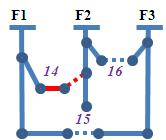
\includegraphics[width=0.2\paperwidth]{OtherImages/reconf.jpg}
\end{minipage}%
\begin{minipage}[!h]{0.25\paperwidth}
  \centering
  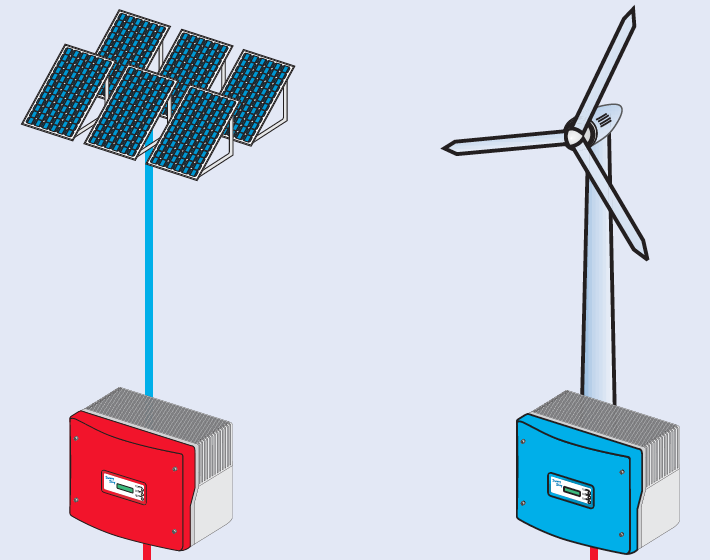
\includegraphics[width=0.2\paperwidth]{OtherImages/VVC.png}
\end{minipage}%
\begin{minipage}[!h]{0.25\paperwidth}
  \centering
  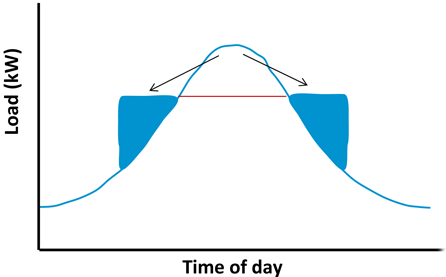
\includegraphics[width=0.2\paperwidth]{OtherImages/LR.png}
\end{minipage}%
\begin{minipage}[!h]{0.25\paperwidth}
  \centering
  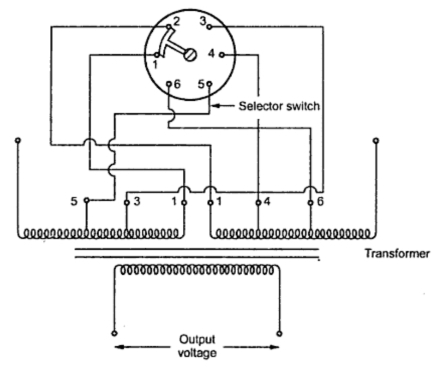
\includegraphics[width=0.2\paperwidth]{OtherImages/OLTC.jpeg}
\end{minipage}
{\footnotesize \textcopyright\ pro-NERDS, SunValley, gov.com.au, wikipedia}
\end{changemargin}    
\end{frame}

% ----------------------------------------------------------------------

\begin{frame}
  {The Algorithm}{Economic Models}
\begin{changemargin}{-0.8cm}{-0.8cm}
  \vspace{0.3cm}
  \begin{itemize}
  \item Switching:
  \begin{align*} 
    Cost/switching&=\frac{C_{sw}}{n_{sw}}+ C_{OM}+C_{log}\\
    C_{OM}&=c \cdot f(t_{sw})
  \end{align*}
  \item OLTC:
  \begin{align*} 
    Cost/operation&=\frac{C_{OLTC}}{n_{op}}+ C_{OM}+C_{log}\\
    C_{OM}&=c \cdot f(t_{op})
  \end{align*}
  \vspace{0.2cm}
  \item Models for Load Reduction, VVC, and Violations are more difficult to develop.
  \end{itemize}

  \vspace{0.3cm}
  \centering
  \adjustbox{max width=0.4\paperwidth}{
  \begin{tabular}{cc}
  % \hline\hline
  \rowcolor{gray!15}
  Switching Operation & $300$ \euro \\
  % \hline
  Load Reduction & $6$ \euro/MWh \\
  % \hline
  \rowcolor{gray!15}
  OLTC Operation & $20$ \euro/Tap Change \\
  % \hline
  VVC & $132.9$ \euro/MWh \\
  % \hline
  \rowcolor{gray!15}
  Violations & $500$ \euro/violation \\
  % \hline
  \end{tabular}
  }

\end{changemargin}
\end{frame}

% ----------------------------------------------------------------------

\begin{frame}
  {The Algorithm}{Components}
    \vspace{0.3cm}
    \begin{figure}[!h]
    \centering
    \resizebox{!}{0.45\paperwidth}{%
    \begin{tikzpicture}

    \pgfdeclarelayer{background}
    \pgfdeclarelayer{foreground}
    \pgfsetlayers{background,main,foreground}

    \tikzstyle{lcomp}=[draw, fill=blue!20, text width=5em, 
        text centered, minimum height=2.5em,text centered]

    \tikzstyle{ann} = [above, text width=5em]

    \tikzstyle{program} = [lcomp, text width=6em, fill=red!20, 
        minimum height=6em, minimum width=10em, rounded corners,text centered, drop shadow]

    \tikzstyle{global} = [lcomp, text width=6em,
        fill=green!20, minimum height=6em, minimum width=8em, rounded corners,text centered, drop shadow]

    \tikzstyle{reconf} = [lcomp, text width=8em, fill=gray!10, 
        minimum height=4em, minimum width=8em, rounded corners,text centered, drop shadow]

    \tikzstyle{lf} = [lcomp, text width=8em, fill=yellow!20, 
        minimum height=4em, minimum width=8em, rounded corners,text centered, drop shadow]

    \tikzstyle{local} = [draw, circle, text width=3em, fill=blue!20,
        minimum height=3em, minimum width=3em, text centered, circular drop shadow]

    \tikzstyle{blank} = [node distance=1cm,minimum width=-1cm]

    \tikzstyle{vecArrow} = [thick, decoration={markings,mark=at position 0 with {\arrowreversed[semithick]{open triangle 60}},mark=at position
       1 with {\arrow[semithick]{open triangle 60}}},
       double distance=1.4pt, shorten >= 5.5pt, shorten <= -5.5pt,
       preaction = {decorate},
       postaction = {draw,line width=1.4pt, white,shorten >= 4.5pt, shorten <= 4.5pt}]
    \tikzstyle{innerWhite} = [semithick, white,line width=1.4pt, shorten >= 4.5pt, shorten <= -7pt]


	% Main Program
    \node [program] (prog) {Main Program};

    % Reconfiguration
    \node [blank,right of=prog, node distance=1cm] (b1) {};
    \node [reconf,below of=prog, node distance=3.5cm] (rec) {Reconfiguration Algorithm};
    \node [reconf, right of=rec,node distance=5cm] (recdb) {Reconfiguration Database};
    \node [blank, left of=rec, node distance=2cm] (b5) {};

    % Load Flow
    \node [lf, above of=prog, node distance=3cm] (ld) {Load Flow};

    % Local Management
    \node [blank, below of=prog, node distance=3cm] (b2) {};
    \node [local, left of=prog, node distance=4cm] (lr) {LR};
    \node [local, left of=lr, node distance=2cm] (vvc) {VVC};
    \node [blank, left of=lr, node distance=1cm] (b3) {};
    \node [blank, right of=lr, node distance=1cm] (b4) {};
    \node [local, below of=b3, node distance=1.5cm] (oltc) {OLTC};
    \node [blank, above of=oltc, node distance=3cm] (lmg) {\large Local Management};

    % Global Management
    \node [global,right of=prog, node distance=5cm] (gm) {Global Management};

    \begin{pgfonlayer}{background}
        \path (vvc.west)+(-0.5,1.8) node (a) {};
        \path (oltc.south -| lr.east)+(+0.5,-0.2) node (b) {};
        \path[fill=blue!10,rounded corners, draw=black!50, dashed]
            (a) rectangle (b);

        \path (rec.north west)+(-0.5,0.5) node (c) {};
        \path (recdb.south east)+(+0.5,-0.5) node (d) {};
        \path[fill=gray!05,rounded corners, draw=black!50, dashed]
            (c) rectangle (d);
    \end{pgfonlayer}

    \draw[vecArrow] (prog.north)+(0,0.4) to (ld);
    \draw[innerWhite] (prog.north)+(0,0.4) to (ld);

    \draw[vecArrow] (lmg.north)+(0,0.45) |- (ld);
    \draw[innerWhite] (lmg.north)+(0,0.45) |- (ld);

    \draw[vecArrow] (gm.north)+(0,0.4) |- (ld);
    \draw[innerWhite] (gm.north)+(0,0.4) |- (ld);

	\draw[vecArrow] (b4)+(0.45,0) to (prog);
    \draw[innerWhite] (b4)+(0.45,0) to (prog);

    \draw[vecArrow] (prog.east)+(0.4,0) to (gm);
    \draw[innerWhite] (prog.east)+(0.4,0) to (gm);

	\draw[vecArrow] (rec.north)+(0,0.9) to (prog.south);
    \draw[innerWhite] (rec.north)+(0,0.9) to (prog.south);

    \draw[vecArrow] (recdb.north)+(0,0.9) to (gm.south);
    \draw[innerWhite] (recdb.north)+(0,0.9) to (gm.south);

    \draw[vecArrow] (gm.east)+(0.4,0) to node {} +(1.2,0) to node {} +(1.2,-5) to node {} +(-11.2,-5) to node {} +(-11.2,-2.25);
    \draw[innerWhite] (gm.east)+(0.4,0) to node {} +(1.2,0) to node {} +(1.2,-5) to node {} +(-11.2,-5) to node {} +(-11.2,-2.25);
    
\end{tikzpicture}
    }
    \end{figure}
    \vspace{-0.3cm}
    {\footnotesize Legend: VVC: Voltage VAr Control, LR: Load Reduction, OLTC: On-Load Tap Changing}
\end{frame}

% ----------------------------------------------------------------------

\begin{frame}
  {The Algorithm}{Components - Reconfiguration}
  \begin{changemargin}{-0.9cm}{-1cm}

  \begin{minipage}[H]{0.35\paperwidth}
  \centering
  \vspace{0.1cm}
  Multi-Objective Reconfiguration\\
  \vspace{1.1cm}
  {\tiny
    \def\firstcircle{(90:0.6cm) circle (1.5cm)}
    \def\secondcircle{(210:1.9cm) circle (1.5cm)}
    \def\thirdcircle{(330:1.9cm) circle (1.5cm)}
    \def\fourthcircle{(90:-2.6cm) circle (1.5cm)}

      \begin{tikzpicture}[scale=0.6]
      \begin{scope}[fill opacity=0.4]
          \fill[red] \firstcircle;
          \fill[green] \secondcircle;
          \fill[blue] \thirdcircle;
          \fill[yellow] \fourthcircle;
      \end{scope}
          \draw \firstcircle node[text=black,above=0.05cm] {Branch Current};
          \draw \secondcircle node [text=black, left=-0.3cm] {Voltage};
          \draw \thirdcircle node [text=black,right=-0.3cm] {Losses};
          \draw \fourthcircle node [text=black,below=0.05cm]{Feeder Current};
      \end{tikzpicture}
  }%
  \end{minipage}%
  \begin{minipage}[H]{0.65\paperwidth}
  \centering
  \begin{itemize}
  \item Branch exchange based method with pre-selection
  \item Membership Functions for Each Objective:\\
  \vspace{0.3cm}
  \resizebox{0.5\paperwidth}{!}{%
    \centering
    \begin{tabular}{c}
      \cellcolor{blue!25}\\
      \cellcolor{blue!25}{$\!\begin{aligned} 
        x_i &= \frac{PLOSS(i)}{PLOSS0} & &i= 1,2,N_k\\
        \mu L_i &= \frac{(x_{max}-x_i)}{(x_{max}-x_{min})} & &\mathrm{for}\ x_{min}<x_i<x_{max}\\
        \mu L_i &=0 & &\mathrm{for}\ x_i\le x_{min}\\
        \mu L_i &=1 & &\mathrm{for}\ x_i\ge x_{max}
      \end{aligned}$}\\
      \cellcolor{blue!25}\\
    \end{tabular}
  }
  \vspace{0.3cm}
  \item Fuzzy min-max principle for finding branch to exchange
  \item Reconfiguration database based on ``maximum'' conditions
  \end{itemize}
  \end{minipage}

  \end{changemargin}
\end{frame}

% ----------------------------------------------------------------------

\begin{frame}
  {The Algorithm}{Components - Local Management}

   To manage ``local'' violations in distribution networks for the hour when it is launched.\\
   \vspace{0.2cm}
   % \begin{tabular}{c|c}
   % \textbf{Voltage Violations} & \textbf{Current Violations}\\
   % When $V<0.95pu$ or $V>1.05pu$ & When $I>I_{max}$\\
   % Solution: Use nearby nodes to improve voltage profile & Solution: Use downstream nodes to try reduce line current\\
   % Objective function: $f=abs(V-(0.95+c)$ & Objective function: $f=abs(I_{max}-(I+c))$\\
   % \end{tabular}
   \begin{minipage}[!h]{0.45\paperwidth}
    \begin{block}{Voltage Violations}
      \begin{itemize}
        \item When $V<0.95pu$ or $V>1.05pu$
        \item Solution: Use nearby nodes to improve voltage profile
        \item Objective function: $f=abs(V-(0.95+c))$
      \end{itemize}
    \end{block}
   \end{minipage}%
   \begin{minipage}[!h]{0.45\paperwidth}
   \centering
    \begin{alertblock}{Current Violations}
      \begin{itemize}
        \item When $I>I_{max}$
        \item Solution: Use downstream nodes to try reduce line current
        \item Objective function: $f=abs(I_{max}-(I+c))$
      \end{itemize}
    \end{alertblock}
   \end{minipage}

   \begin{itemize}
    \item When both current and voltage violations exist, consider both sets of nodes, $f=abs(V-(0.95+c))+abs(I_{max}-(I+c))$
    \item Once done, check if $C_{spent} \ge C_{org}$, if yes, do not optimize.
    \item Return solution to calling function.
   \end{itemize}
\end{frame}

% ----------------------------------------------------------------------

\begin{frame}
  {The Algorithm}{Components - Global Management}
  \begin{changemargin}{-1cm}{-0.8cm}
  \centering
    \begin{tikzpicture}[-,sibling distance=8cm]
      \small
      \node {\texttt{Global Management (hour h)}} [edge from parent fork down]
      child {node {\texttt{With Reconfiguration}}}
      child {node {\texttt{Without Reconfiguration}}};
    \end{tikzpicture}\\
  \vspace{0.5cm}
  \begin{minipage}[!h]{0.5\paperwidth}
  \centering
    \begin{itemize}
      \item At hour \emph{h}, perform reconfiguration, and globally optimize using LM functions
      \item From hour \emph{h+1} to end of the day, check for violations
      \item Classify violations found and launch the respective management function
      \item At the end of the day, calculate overall costs\\and feed it back to calling function
    \end{itemize}
  \end{minipage}%
  \begin{minipage}[!h]{0.5\paperwidth}
  \centering
    \begin{itemize}
      \item At hour \emph{h}, use only LM functions to optimize globally
      \item From hour \emph{h+1} to end of the day, check for violations
      \item Classify violations found and launch the respective management function
      \item At the end of the day, calculate overall costs\\and feed it back to calling function
    \end{itemize}
  \end{minipage}
  \end{changemargin}
\end{frame}

% ----------------------------------------------------------------------

\begin{frame}
  {The Algorithm}{Working}
    \vspace{0.6cm}
    \begin{changemargin}{-1cm}{-1cm}
    \begin{figure}[!h]
    \centering
    \resizebox{0.95\paperwidth}{!}{%
    \begin{tikzpicture}[node distance = 1.5cm, auto]
\small

\tikzstyle{blank} = [node distance=1cm,minimum width=-1cm]
\tikzstyle{dot} = [draw, shape=circle, fill=red, minimum size=3mm,scale=0.5]
\tikzstyle{line} = [draw, -latex']


\node [blank] (start) {Start (0h)};
\node [blank, above of=start, node distance=0.25cm] (text1) {};

\node [blank, right of=text1, node distance=3cm] (l1) {Local Vio. (h1)};
% Because Scale = 0.5
\node [dot,right of=start, node distance=6cm] (d1) {};

\node [blank, right of=text1, node distance=5.5cm] (g1) {Global Vio. (h2)};
\node [dot,right of=start, node distance=11cm] (d2) {};

\node [blank, right of=text1, node distance=8cm] (l2) {Local Vio. (h3)};
\node [dot,right of=start, node distance=16cm] (d3) {};

\node [blank, right of=text1, node distance=12cm] (l3) {Local Vio. (h4)};
\node [dot,right of=start, node distance=24cm] (d4) {};

\node [blank, right of=start, node distance=15cm] (end1) {Cost = C1};

\node [blank, below of=end1, node distance=2cm] (end2) {Cost = C2};
\node [blank, above of=end2, node distance=0.25cm] (text2) {};

\node [blank, below of=end2, node distance=2cm] (end3) {Cost = C3};
\node [blank, above of=end3, node distance=0.25cm] (text3) {};

\node [blank, below of=end3, node distance=2cm] (end4) {Cost = C4};
\node [blank, above of=end4, node distance=0.25cm] (text4) {};

\node [blank, left of=text3, node distance=8cm] (l4) {Local Vio. (h5)};
\node [dot,left of=end3, node distance=16cm] (d5) {};

\node [blank, left of=text3, node distance=6cm] (g2) {Global Vio. (h6)};
\node [dot,left of=end3, node distance=12cm] (d6) {};

\node [blank, left of=text3, node distance=2cm] (l5) {Local Vio. (h7)};
\node [dot,left of=end3, node distance=4cm] (d7) {};

\node [blank, left of=text4, node distance=3.5cm] (l6) {Local Vio. (h8)};
\node [dot,left of=end4, node distance=7cm] (d8) {};

\path [line] (start) -- (end1);
\path [line] ($(d2.south)!0.5!(d2.north)$) |- (end3);
\path [line] ($(d4.south)!0.5!(d4.north)$) |- (end2);
\path [line] ($(d6.south)!0.5!(d6.north)$) |- (end4);

\end{tikzpicture}
    }
    \end{figure}
    \end{changemargin}
\end{frame}

% ----------------------------------------------------------------------

% \begin{frame}
%   {The Algorithm}{Working}
%   \centering

%   \begin{tikzpicture}
%   \draw (0,0) -- (11.5,0);
%   \draw[snake=ticks,segment length=0.5cm] (0,0) -- (11.5,0);
%   \end{tikzpicture}
% \end{frame}


% ----------------------------------------------------------------------
%                             Results
% ----------------------------------------------------------------------

\section
  {Results \& Conclusions}

\begin{frame}<handout:0>
  {}{}
  \begin{changemargin}{-1cm}{-1cm}
  \centering
  {\Huge \color{evolvdso} Part IV\\\ \\Results \& Conclusions}
  \end{changemargin}
\end{frame}

\begin{frame}
  {Initial Results}{Why ``Maximum'' Condition was Chosen}
\begin{changemargin}{-1cm}{-1cm}
\centering
\vspace{0.35cm}
  \begin{minipage}[!h]{0.5\paperwidth}
    \begin{figure}[!h]
      \centering
      PREDIS Network
      \setlength\figureheight{3.5cm}
      \setlength\figurewidth{0.35\paperwidth}
      % This file was created by matlab2tikz v0.4.6 running on MATLAB 8.2.
% Copyright (c) 2008--2014, Nico Schlömer <nico.schloemer@gmail.com>
% All rights reserved.
% Minimal pgfplots version: 1.3
% 
% The latest updates can be retrieved from
%   http://www.mathworks.com/matlabcentral/fileexchange/22022-matlab2tikz
% where you can also make suggestions and rate matlab2tikz.
% 
\begin{tikzpicture}

\begin{axis}[%
width=\figurewidth,
height=\figureheight,
scale only axis,
xmin=0,
xmax=24,
xtick={ 0,  4,  8, 12, 16, 20, 24},
xminorticks=true,
xlabel={Time (hour)},
x label style={at={(0.5,0.07)},anchor=north},
ymin=0,
ymax=1200,
ylabel={Losses (kW)},
y label style={at={(0.1,0.8)},anchor=east},
axis x line*=bottom,
axis y line*=left,
legend style={draw=black,fill=white,legend cell align=left, at={(0.5,-0.25)},anchor=north, legend columns=1}
]
\addplot [color=black,solid,line width=0.8pt]
  table[row sep=crcr]{
0	187.470852708396	\\
1	208.073264002775	\\
2	369.453812970541	\\
3	189.718454522433	\\
4	115.418958958224	\\
5	99.2368118293202	\\
6	159.410349961767	\\
7	145.184867621662	\\
8	506.841683410891	\\
9	875.089613674351	\\
10	658.59429508712	\\
11	447.370112257461	\\
12	479.747476017529	\\
13	876.014308683698	\\
14	1025.66991298176	\\
15	793.638695196897	\\
16	522.557408059643	\\
17	731.118595681807	\\
18	188.51698229905	\\
19	375.813228594712	\\
20	452.72643282892	\\
21	132.665389276462	\\
22	458.467025766648	\\
23	545.317597799103	\\
};
\addlegendentry{Original Network};

\addplot [color=blue,solid,line width=0.6pt]
  table[row sep=crcr]{
0	37.0992700523806	\\
1	30.3620650854819	\\
2	66.2180509631016	\\
3	31.8947685828755	\\
4	30.2290766611202	\\
5	23.0552961419536	\\
6	31.2138404230611	\\
7	26.3484341197884	\\
8	58.0183843249205	\\
9	72.6055806268167	\\
10	114.916329089854	\\
11	137.033387593966	\\
12	236.448536160519	\\
13	163.995249077653	\\
14	422.50083042695	\\
15	237.512954802552	\\
16	74.0303685398846	\\
17	85.0306701981773	\\
18	52.1605535837466	\\
19	79.9883240029414	\\
20	76.2800858210899	\\
21	41.59866233307	\\
22	115.253688184083	\\
23	100.458255996627	\\
};
\addlegendentry{Hourly Reconfiguration};

\addplot [color=red,solid,line width=0.6pt]
  table[row sep=crcr]{
0	64.9398184700778	\\
1	42.8598475862435	\\
2	72.6741675204701	\\
3	38.6113857960654	\\
4	40.8545281369965	\\
5	31.3749970536403	\\
6	55.4639759621944	\\
7	38.3979835758413	\\
8	82.2519796794319	\\
9	96.4950188875768	\\
10	108.251613746782	\\
11	142.507497274888	\\
12	281.180085965371	\\
13	173.810111568062	\\
14	717.850282405204	\\
15	424.866794619111	\\
16	79.3950740225591	\\
17	123.329593935162	\\
18	51.0609103975129	\\
19	110.057762182345	\\
20	114.529191965013	\\
21	51.9788980904906	\\
22	208.364036157857	\\
23	151.286743793291	\\
};
\addlegendentry{Avg. Condition Reconfiguration};

\addplot [color=green,solid,line width=0.8pt]
  table[row sep=crcr]{
0	49.9906360840574	\\
1	58.8871181717937	\\
2	112.07616576048	\\
3	57.2916830921991	\\
4	31.5132123372294	\\
5	25.5056433559525	\\
6	33.2242924258097	\\
7	26.3484341197884	\\
8	58.0620198247339	\\
9	78.2954718226647	\\
10	113.37557755238	\\
11	155.029956450251	\\
12	247.599698220103	\\
13	155.961956971143	\\
14	471.862125347108	\\
15	302.633446508699	\\
16	101.021227926196	\\
17	85.0306701981773	\\
18	67.7191842226782	\\
19	80.1910226861102	\\
20	76.127792687114	\\
21	60.3880584185895	\\
22	115.253688184083	\\
23	100.458255996627	\\
};
\addlegendentry{Max. Condition Reconfiguration};

\end{axis}
\end{tikzpicture}%
    \end{figure}
  \end{minipage}%
  \begin{minipage}[!h]{0.5\paperwidth}
    \begin{figure}[!h]
      \centering
      Rural Network
      \setlength\figureheight{3.5cm}
      \setlength\figurewidth{0.35\paperwidth}
      % This file was created by matlab2tikz v0.4.6 running on MATLAB 8.2.
% Copyright (c) 2008--2014, Nico Schlömer <nico.schloemer@gmail.com>
% All rights reserved.
% Minimal pgfplots version: 1.3
% 
% The latest updates can be retrieved from
%   http://www.mathworks.com/matlabcentral/fileexchange/22022-matlab2tikz
% where you can also make suggestions and rate matlab2tikz.
% 
\begin{tikzpicture}

\begin{axis}[%
width=\figurewidth,
height=\figureheight,
scale only axis,
xmin=0,
xmax=25,
xlabel={Time (hour)},
ymin=10,
ymax=110,
ylabel={Losses (kW)},
axis x line*=bottom,
axis y line*=left,
legend style={draw=black,fill=white,legend cell align=left, at={(0.5,-0.25)},anchor=north, legend columns=2}
]
\addplot [color=black,solid,line width=1.0pt]
  table[row sep=crcr]{
0	36.0418933408924	\\
1	28.4382759081625	\\
2	26.1215707561308	\\
3	21.6061502667575	\\
4	24.3378452311177	\\
5	22.4855092514709	\\
6	23.0639450119174	\\
7	40.4945348436625	\\
8	14.1245722984627	\\
9	15.7413514465241	\\
10	36.0505152919788	\\
11	51.0115231011965	\\
12	29.4802184601339	\\
13	39.5355852743295	\\
14	29.7385119880372	\\
15	16.8690444893987	\\
16	25.7830091609484	\\
17	27.5769625406691	\\
18	87.9169828226134	\\
19	100.697324204575	\\
20	100.968451139209	\\
21	93.5993669897117	\\
22	59.0483117906493	\\
23	49.0753737355887	\\
};
\addlegendentry{Original};

\addplot [color=blue,solid,line width=1.0pt]
  table[row sep=crcr]{
0	29.8637103345656	\\
1	22.6373141949504	\\
2	19.7053601216957	\\
3	16.4116305583722	\\
4	19.9512907898475	\\
5	17.8499022501022	\\
6	19.0806292192391	\\
7	33.3403060085935	\\
8	10.5720864610383	\\
9	11.7742154093067	\\
10	28.7151303060595	\\
11	40.6460576985657	\\
12	24.2471780796827	\\
13	28.0464514021789	\\
14	23.6915321890768	\\
15	13.4226343066141	\\
16	19.3640127836298	\\
17	19.1918976858241	\\
18	66.8954526444188	\\
19	76.5895757427226	\\
20	84.05212486573	\\
21	80.5586657204271	\\
22	49.9103584995042	\\
23	38.1359877287935	\\
};
\addlegendentry{Hourly};

\addplot [color=green,solid,line width=1.0pt]
  table[row sep=crcr]{
0	30.33283203427	\\
1	22.6457056608559	\\
2	20.410797428414	\\
3	17.3330171038094	\\
4	19.9647379664375	\\
5	18.2410594376881	\\
6	19.7722112580778	\\
7	34.1892141350708	\\
8	11.31841625136	\\
9	13.0219548340645	\\
10	30.4078070191116	\\
11	42.7390997019406	\\
12	26.7234420206353	\\
13	28.7140542611941	\\
14	24.9670422070891	\\
15	15.4787399277226	\\
16	19.6070819128896	\\
17	21.7712802323267	\\
18	65.2550219622372	\\
19	77.6377164938191	\\
20	84.748323595718	\\
21	79.8176392074934	\\
22	50.4810296829195	\\
23	38.5286836528209	\\
};
\addlegendentry{Max.};

\addplot [color=red,solid,line width=1.0pt]
  table[row sep=crcr]{
0	29.9306202161709	\\
1	22.6373141949504	\\
2	20.768359308449	\\
3	17.09896311507	\\
4	20.3734343013745	\\
5	17.9245135558709	\\
6	20.0970300854536	\\
7	34.0015048699116	\\
8	11.4050399073212	\\
9	13.0512798247813	\\
10	30.4154024320413	\\
11	42.7212608799521	\\
12	26.7355418210358	\\
13	28.7171750207743	\\
14	24.9881230319193	\\
15	15.5092111353933	\\
16	19.6298876792561	\\
17	21.7633368776976	\\
18	65.5661067446867	\\
19	76.8487929385442	\\
20	84.5216131595583	\\
21	80.0031725967276	\\
22	50.3306035220241	\\
23	38.5175153519735	\\
};
\addlegendentry{Avg.};

\end{axis}
\end{tikzpicture}%
    \end{figure}
  \end{minipage}
\end{changemargin}
\end{frame}

% ----------------------------------------------------------------------

\begin{frame}
  {Results}{Methodology}

  \begin{itemize}
  \item Both networks were tested with the two load models.\\\ \\

  \item Two initial configurations were used: the original, and the 24 hour optimal configurations.\\\ \\ \pause

    \vspace{0.5cm} 
    \begin{tabular}{cc}
    \rowcolor{gray!25}
    \multicolumn{2}{c}{Output Variables}\\
    \hline
    \rowcolor{gray!15}
    Money Spent without Optimization & Money Spent with Optimization\\
    Load Reduction effected & DRES VVC Outputs\\
    \rowcolor{gray!15}
    Number of Switching Operations & Number of OLTC Operations\\
    Loss Curves over the 24h period & Complete Bus Voltage Profiles\\
    \rowcolor{gray!15}
    Violations in the Network & Final Line and Bus statuses for every hour\\
    \hline
    \end{tabular}

  \end{itemize}

\end{frame}

% ----------------------------------------------------------------------

\begin{frame}
  {Results}{PREDIS Network - Load Model A}
  \begin{changemargin}{-1cm}{-1cm}
  \centering
  \vspace{0.4cm}
  % \begin{minipage}[!h]{0.65\paperwidth}
    \begin{minipage}[!h]{0.5\paperwidth}
    \centering
      \setlength\figureheight{3.5cm}
      \setlength\figurewidth{0.35\paperwidth}
      % This file was created by matlab2tikz v0.4.6 running on MATLAB 8.2.
% Copyright (c) 2008--2014, Nico Schlömer <nico.schloemer@gmail.com>
% All rights reserved.
% Minimal pgfplots version: 1.3
% 
% The latest updates can be retrieved from
%   http://www.mathworks.com/matlabcentral/fileexchange/22022-matlab2tikz
% where you can also make suggestions and rate matlab2tikz.
% 
\begin{tikzpicture}

\begin{axis}[%
width=\figurewidth,
height=\figureheight,
scale only axis,
xmin=1,
xmax=24,
xlabel={Time (hour)},
x label style={at={(0.5,0.09)},anchor=north},
ymin=0,
ymax=1200,
ylabel={Losses (kW)},
y label style={at={(0.1,0.8)},anchor=east},
axis x line*=bottom,
axis y line*=left,
legend style={draw=black,fill=white,legend cell align=left, at={(0.5,-0.17)},anchor=north, legend columns=1}
]
\addplot [color=red,solid,line width=1.0pt,mark=asterisk,mark options={solid}]
  table[row sep=crcr]{
0   273.291098533993    \\
1   282.883988799185    \\
2   484.457090834875    \\
3   280.795992600733    \\
4   202.2770567744  \\
5   185.434351023359    \\
6   231.830509016609    \\
7   222.3258291977  \\
8   387.721498842253    \\
9   701.434470847533    \\
10  470.267423390158    \\
11  325.165024492763    \\
12  363.191877673265    \\
13  641.489871778722    \\
14  888.203974469809    \\
15  633.128372293215    \\
16  340.033853735636    \\
17  510.1638446975  \\
18  142.05734485522 \\
19  359.040838567293    \\
20  526.98651847653 \\
21  186.150392103251    \\
22  601.438001672017    \\
23  593.787493021791    \\
};
\addlegendentry{Unoptimized Network};

\addplot [color=blue,solid,line width=1.0pt,mark=square,mark options={solid}]
  table[row sep=crcr]{
0   273.291098533998    \\
1   282.883988799187    \\
2   121.660248981492    \\
3   60.2455848765004    \\
4   41.7021073032459    \\
5   33.6334325365006    \\
6   34.6982298451592    \\
7   34.0823667428797    \\
8   45.3322515257204    \\
9   62.591412973606 \\
10  116.66865036906 \\
11  172.503635456776    \\
12  254.273529194148    \\
13  144.499489562683    \\
14  461.103483208029    \\
15  282.8054247793  \\
16  78.7555159221326    \\
17  69.0014456573268    \\
18  100.239925076984    \\
19  116.408640259746    \\
20  104.851189839822    \\
21  105.735991912262    \\
22  144.591433824576    \\
23  105.81457186743 \\
};
\addlegendentry{Begin with Original Configuration};


\end{axis}
\end{tikzpicture}%
    \end{minipage}%
    \begin{minipage}[!h]{0.5\paperwidth}
    \centering
      \setlength\figureheight{3.5cm}
      \setlength\figurewidth{0.35\paperwidth}
      % This file was created by matlab2tikz v0.4.6 running on MATLAB 8.2.
% Copyright (c) 2008--2014, Nico Schlömer <nico.schloemer@gmail.com>
% All rights reserved.
% Minimal pgfplots version: 1.3
% 
% The latest updates can be retrieved from
%   http://www.mathworks.com/matlabcentral/fileexchange/22022-matlab2tikz
% where you can also make suggestions and rate matlab2tikz.
% 
\begin{tikzpicture}

\begin{axis}[%
width=\figurewidth,
height=\figureheight,
scale only axis,
xmin=1,
xmax=24,
xlabel={Time (hour)},
ymin=0,
ymax=1200,
ylabel={Losses (kW)},
axis x line*=bottom,
axis y line*=left,
legend style={draw=black,fill=white,legend cell align=left, at={(0.5,-0.25)},anchor=north, legend columns=1}
]
\addplot [color=red,solid,line width=1.0pt,mark=asterisk,mark options={solid}]
  table[row sep=crcr]{
0	188.746701154496	\\
1	209.886341768802	\\
2	382.175666944748	\\
3	190.842288058898	\\
4	113.776708443172	\\
5	97.2160251100973	\\
6	159.786331148939	\\
7	145.651392202956	\\
8	548.793623806954	\\
9	987.249704059046	\\
10	773.922382207043	\\
11	528.235957184667	\\
12	574.127076949348	\\
13	1034.1118869356	\\
14	1195.76001141325	\\
15	919.850020005017	\\
16	588.012533715604	\\
17	823.932458528714	\\
18	200.901710137755	\\
19	402.172630418562	\\
20	477.117123227819	\\
21	134.410636291632	\\
22	476.789352821111	\\
23	567.306772548803	\\
};
\addlegendentry{Unoptimized Network};

\addplot [color=green,solid,line width=1.0pt,mark=triangle,mark options={solid}]
  table[row sep=crcr]{
0	72.3492505641701	\\
1	77.4323908613678	\\
2	167.801061512578	\\
3	88.3470764671671	\\
4	108.317767954803	\\
5	72.8953730080389	\\
6	49.7883287157247	\\
7	108.855711974737	\\
8	176.842817390085	\\
9	153.32125536084	\\
10	149.754231931823	\\
11	204.219141142198	\\
12	309.94071017332	\\
13	197.546156690215	\\
14	531.617798079534	\\
15	331.158583579175	\\
16	87.7149676740574	\\
17	72.5105476091836	\\
18	57.2585205291104	\\
19	68.6014642063748	\\
20	62.5798090518936	\\
21	43.1983592887195	\\
22	102.851266201812	\\
23	110.99908747981	\\
};
\addlegendentry{Begin with Optimal Configuration};


\end{axis}
\end{tikzpicture}%
    \end{minipage}\\
  % \end{minipage}
  % \vspace{0.4cm}
  % \resizebox{0.9\paperwidth}{!}{%}
  %   \begin{tabular}{cccc}
  %   \rowcolor{gray!25}
  %   & \textbf{Unoptimized Network} & \textbf{Begin With Original Configuraiton} & \textbf{Begin With Optimal Configuration}\\
  %   \hline
  %   Losses & & & \\
  %   \hline
  %   \end{tabular}
  % }
  \end{changemargin}
\end{frame}

% ----------------------------------------------------------------------

\begin{frame}
  {Results}{PREDIS Network - Load Model A}
  \begin{changemargin}{-1cm}{-1cm}
  \centering
  \vspace{0.4cm}
  % \begin{minipage}[!h]{0.65\paperwidth}
    \begin{minipage}[!h]{0.5\paperwidth}
    \centering
      \setlength\figureheight{3.5cm}
      \setlength\figurewidth{0.35\paperwidth}
      % This file was created by matlab2tikz v0.4.6 running on MATLAB 8.2.
% Copyright (c) 2008--2014, Nico Schlömer <nico.schloemer@gmail.com>
% All rights reserved.
% Minimal pgfplots version: 1.3
% 
% The latest updates can be retrieved from
%   http://www.mathworks.com/matlabcentral/fileexchange/22022-matlab2tikz
% where you can also make suggestions and rate matlab2tikz.
% 
\begin{tikzpicture}
\tikzset{mark size=1}
\begin{axis}[%
width=\figurewidth,
height=\figureheight,
scale only axis,
xmin=1,
xmax=24,
xlabel={Time (hour)},
x label style={at={(0.5,0.08)},anchor=north},
ymin=0.8,
ymax=1.15,
ytick={0.8,0.9,0.95,1,1.05,1.1},
ylabel={Voltages (pu)},
y label style={at={(0.09,0.8)},anchor=east},
title style={align=center, at={(0.5,0.7)}},
title={Begin with\\ [0.25ex]Original Configuration},
axis x line*=bottom,
axis y line*=left,
legend style={draw=black,fill=white,legend cell align=left, at={(0.5,-0.17)},anchor=north, legend columns=2}
]
\addplot [color=green,dashed,line width=0.6pt,mark=asterisk,mark options={solid}]
  table[row sep=crcr]{
0	0.982338456972398	\\
1	0.989137780079637	\\
2	0.992703787134075	\\
3	0.990559819229489	\\
4	0.98570902981714	\\
5	0.986995142168046	\\
6	0.980554612440615	\\
7	0.980833270894023	\\
8	0.960080799926757	\\
9	0.95524171138273	\\
10	0.949547820073847	\\
11	0.958229646264734	\\
12	0.962472572853943	\\
13	0.952635747000472	\\
14	0.958969812659031	\\
15	0.960110512716527	\\
16	0.957975784323266	\\
17	0.94829276142638	\\
18	0.9698906445541	\\
19	0.960831225963349	\\
20	0.964476563623062	\\
21	0.977753958841346	\\
22	0.965402509018886	\\
23	0.988135068014865	\\
};
\addlegendentry{Original Avg};

\addplot [color=red,dashed,line width=0.6pt,mark=triangle,mark options={solid}]
  table[row sep=crcr]{
0	0.935885019564693	\\
1	0.939643416338232	\\
2	0.947933146415685	\\
3	0.9461777443953	\\
4	0.951132609363904	\\
5	0.953524113184857	\\
6	0.944720249741136	\\
7	0.943816597346418	\\
8	0.881267148880854	\\
9	0.847969548495464	\\
10	0.863018599275384	\\
11	0.90712418847755	\\
12	0.905315693181888	\\
13	0.841662782879085	\\
14	0.842209546221409	\\
15	0.849221741768934	\\
16	0.863026029625246	\\
17	0.848741610544043	\\
18	0.915126243996083	\\
19	0.897622663439686	\\
20	0.89555904495215	\\
21	0.944454026025918	\\
22	0.907348715898211	\\
23	0.917355872206259	\\
};
\addlegendentry{Original Min};

\addplot [color=blue,dashed,line width=0.6pt,mark=+,mark options={solid}]
  table[row sep=crcr]{
0	1.00168274336364	\\
1	1.0237649855227	\\
2	1.06262012953497	\\
3	1.02997558424276	\\
4	1.00168274336364	\\
5	1.00168274336364	\\
6	1.00168274336364	\\
7	1.00168274336364	\\
8	1.00168274336363	\\
9	1.00525225756647	\\
10	1.01884109704913	\\
11	1.02186284819987	\\
12	1.02451696057379	\\
13	1.02131749541946	\\
14	1.02717968604658	\\
15	1.02258413962856	\\
16	1.00168274336363	\\
17	1.00168274336363	\\
18	1.00168274336363	\\
19	1.00168274336363	\\
20	1.00168274336363	\\
21	1.00168274336363	\\
22	1.00168274336363	\\
23	1.06858893093808	\\
};
\addlegendentry{Original Max};

\addplot [color=green,solid,line width=0.6pt,mark=asterisk,mark options={solid}]
  table[row sep=crcr]{
0	0.982338456972398	\\
1	0.990464023557581	\\
2	0.991869527196084	\\
3	0.991208614952886	\\
4	0.990138974503414	\\
5	0.990695423712349	\\
6	0.988238630423826	\\
7	0.988208321867238	\\
8	0.978180131989974	\\
9	0.973754225380391	\\
10	0.976288453584446	\\
11	0.976500266581573	\\
12	0.978547200089105	\\
13	0.981238645675447	\\
14	0.981337167239773	\\
15	0.979765455312702	\\
16	0.977288157568904	\\
17	0.973447011717444	\\
18	0.979376834322476	\\
19	0.976860352631207	\\
20	0.980012105986901	\\
21	0.984646866951606	\\
22	0.980760904179698	\\
23	0.991715080909499	\\
};
\addlegendentry{Optimal Avg};

\addplot [color=red,solid,line width=0.6pt,mark=triangle,mark options={solid}]
  table[row sep=crcr]{
0	0.935885019564693	\\
1	0.969020327115041	\\
2	0.971245022588594	\\
3	0.970490926371657	\\
4	0.97163633583066	\\
5	0.973684453070567	\\
6	0.973428304588147	\\
7	0.977297859066955	\\
8	0.959828634586379	\\
9	0.949961670254353	\\
10	0.954787137618888	\\
11	0.954156591405115	\\
12	0.949401605061437	\\
13	0.955138240537614	\\
14	0.953776560913987	\\
15	0.953728120832429	\\
16	0.953201156771066	\\
17	0.952100312944082	\\
18	0.957186468629564	\\
19	0.957328349475766	\\
20	0.962849077333358	\\
21	0.970709202176027	\\
22	0.949613417412595	\\
23	0.973597584830785	\\
};
\addlegendentry{Optimal Min};

\addplot [color=blue,solid,line width=0.6pt,mark=+,mark options={solid}]
  table[row sep=crcr]{
0	1.00168274336364	\\
1	1.0059302093923	\\
2	1.02075522883851	\\
3	1.00884612825641	\\
4	1	\\
5	1	\\
6	1	\\
7	1	\\
8	1	\\
9	1	\\
10	1	\\
11	1	\\
12	1	\\
13	1	\\
14	1.04125264245311	\\
15	1.03690578858613	\\
16	1.00643478493281	\\
17	1	\\
18	1.00111623037449	\\
19	1	\\
20	1	\\
21	1	\\
22	1	\\
23	1.01083327069291	\\
};
\addlegendentry{Optimal Max};

\end{axis}
\end{tikzpicture}%
    \end{minipage}%
    \begin{minipage}[!h]{0.5\paperwidth}
    \centering
      \setlength\figureheight{3.5cm}
      \setlength\figurewidth{0.35\paperwidth}
      % This file was created by matlab2tikz v0.4.6 running on MATLAB 8.2.
% Copyright (c) 2008--2014, Nico Schlömer <nico.schloemer@gmail.com>
% All rights reserved.
% Minimal pgfplots version: 1.3
% 
% The latest updates can be retrieved from
%   http://www.mathworks.com/matlabcentral/fileexchange/22022-matlab2tikz
% where you can also make suggestions and rate matlab2tikz.
% 
\begin{tikzpicture}

\begin{axis}[%
width=\figurewidth,
height=\figureheight,
scale only axis,
xmin=1,
xmax=24,
xlabel={Time (hour)},
ymin=0.8,
ymax=1.15,
ytick={0.8,0.9,0.95,1,1.05,1.1},
ylabel={Voltages (pu)},
title style={align=center, at={(0.5,0.75)}},
title={Begin with\\ [0.25ex]Optimal Configuration},
axis x line*=bottom,
axis y line*=left,
legend style={draw=black,fill=white,legend cell align=left, at={(0.5,-0.25)},anchor=north, legend columns=2}
]
\addplot [color=green,dashed,line width=1.0pt,mark=asterisk,mark options={solid}]
  table[row sep=crcr]{
0	0.97418645718086	\\
1	0.982436615590071	\\
2	0.985977614472308	\\
3	0.983538920758001	\\
4	0.978446169227937	\\
5	0.980388149225668	\\
6	0.975424637507249	\\
7	0.97735311213191	\\
8	0.969258322011489	\\
9	0.969584555838294	\\
10	0.966376331957361	\\
11	0.972871384683681	\\
12	0.977714861077176	\\
13	0.96787703369701	\\
14	0.97350041888514	\\
15	0.974598997143008	\\
16	0.971841254835905	\\
17	0.96215256328127	\\
18	0.972724945180711	\\
19	0.958833977907986	\\
20	0.956678224333835	\\
21	0.96904034290702	\\
22	0.953011484554403	\\
23	0.979207535299228	\\
};
\addlegendentry{Original Avg};

\addplot [color=red,dashed,line width=1.0pt,mark=triangle,mark options={solid}]
  table[row sep=crcr]{
0	0.915592003828552	\\
1	0.921311695118007	\\
2	0.925429728128957	\\
3	0.924449436956124	\\
4	0.928782863073251	\\
5	0.930716552117562	\\
6	0.927010224215227	\\
7	0.926844698697513	\\
8	0.905245598485622	\\
9	0.880343546849075	\\
10	0.901185368130367	\\
11	0.938021418027778	\\
12	0.942033825025743	\\
13	0.885009719495526	\\
14	0.877468499259205	\\
15	0.886391501742796	\\
16	0.901357509302696	\\
17	0.889320292392278	\\
18	0.936464814507733	\\
19	0.909243602330113	\\
20	0.888862343627417	\\
21	0.933181080141931	\\
22	0.889454803993173	\\
23	0.901208447310785	\\
};
\addlegendentry{Original Min};

\addplot [color=blue,dashed,line width=1.0pt,mark=+,mark options={solid}]
  table[row sep=crcr]{
0	1.00144760066773	\\
1	1.02341037058506	\\
2	1.06580754069848	\\
3	1.03191620314533	\\
4	1.00149746778834	\\
5	1.00150744707381	\\
6	1.00150499918152	\\
7	1.00152241807739	\\
8	1.00150031245516	\\
9	1.00379373320167	\\
10	1.0167098643962	\\
11	1.02008378387032	\\
12	1.02328048293521	\\
13	1.01957543377667	\\
14	1.03195419551178	\\
15	1.02651776446284	\\
16	1.00144859418164	\\
17	1.00145137116932	\\
18	1.00138548821537	\\
19	1.00135174260857	\\
20	1.00134656030977	\\
21	1.00135055145129	\\
22	1.0013576555865	\\
23	1.06281043442049	\\
};
\addlegendentry{Original Max};

\addplot [color=green,solid,line width=1.0pt,mark=asterisk,mark options={solid}]
  table[row sep=crcr]{
0	0.976837907659437	\\
1	0.980379769136527	\\
2	0.990556511066244	\\
3	0.988876210512215	\\
4	0.987452461112452	\\
5	0.988547991374539	\\
6	0.98702630712318	\\
7	0.98779316875885	\\
8	0.983891136718197	\\
9	0.981987372778413	\\
10	0.984099527422873	\\
11	0.983532222886173	\\
12	0.985746084807427	\\
13	0.987954010966603	\\
14	0.988267943628302	\\
15	0.987057003174592	\\
16	0.98264410876199	\\
17	0.9794511377837	\\
18	0.980127221175585	\\
19	0.975556702142156	\\
20	0.976716241145118	\\
21	0.980087222495318	\\
22	0.975740791367255	\\
23	0.987169862783849	\\
};
\addlegendentry{Optimal Avg};

\addplot [color=red,solid,line width=1.0pt,mark=triangle,mark options={solid}]
  table[row sep=crcr]{
0	0.912170535543406	\\
1	0.920475671086295	\\
2	0.975251768007297	\\
3	0.974475576055271	\\
4	0.975639413463921	\\
5	0.977251876844773	\\
6	0.975557776359956	\\
7	0.978946890989611	\\
8	0.966254764431064	\\
9	0.963553603067948	\\
10	0.969882056397168	\\
11	0.967362381642357	\\
12	0.963576670625614	\\
13	0.971485852149109	\\
14	0.968133212306428	\\
15	0.96977834307183	\\
16	0.95799598519194	\\
17	0.95771095848635	\\
18	0.955411849971744	\\
19	0.952451680631381	\\
20	0.952144716522555	\\
21	0.956974107556123	\\
22	0.955514645020933	\\
23	0.974664909669098	\\
};
\addlegendentry{Optimal Min};

\addplot [color=blue,solid,line width=1.0pt,mark=+,mark options={solid}]
  table[row sep=crcr]{
0	1.00150214391914	\\
1	1.01292891337217	\\
2	1.01212980503737	\\
3	1	\\
4	1	\\
5	1	\\
6	1	\\
7	1	\\
8	1	\\
9	1	\\
10	1	\\
11	1	\\
12	1	\\
13	1	\\
14	1.04091930629977	\\
15	1.03620859283368	\\
16	1.00532545319908	\\
17	1	\\
18	1.0003641954998	\\
19	1	\\
20	1	\\
21	1	\\
22	1	\\
23	1.00741802737326	\\
};
\addlegendentry{Optimal Max};

\end{axis}
\end{tikzpicture}%
    \end{minipage}\\
  % \end{minipage}
  % \vspace{0.2cm}
  \resizebox{0.9\paperwidth}{!}{%}
    \begin{tabular}{cccc}
    \rowcolor{gray!25}
    & \textbf{Unoptimized Network} & \textbf{Begin With Original Configuraiton} & \textbf{Begin With Optimal Configuration}\\
    \hline
    Minimum Voltage (pu) & $0.8417$ & \cellcolor{green!25}$0.9359$ & $0.9290$\\
    % \rowcolor{gray!15}
    Average Voltage (pu) & $0.9700$ & \cellcolor{green!25}$0.9826$ & $0.9809$\\
    Maximum Voltage (pu) & $1.0686$ & \cellcolor{green!25}$1.0413$ & \cellcolor{green!25}$1.0413$\\
    \hline
    \end{tabular}
  }
  \end{changemargin}
\end{frame}

% ----------------------------------------------------------------------

\begin{frame}
  {Results}{PREDIS Network - Load Model A}
  \begin{changemargin}{-1cm}{-1cm}
  \vspace{0.4cm}
  \centering
    {\tiny%
    \setlength\figureheight{3cm}
    \setlength\figurewidth{0.9\paperwidth}
    % This file was created by matlab2tikz v0.4.6 running on MATLAB 8.2.
% Copyright (c) 2008--2014, Nico Schlömer <nico.schloemer@gmail.com>
% All rights reserved.
% Minimal pgfplots version: 1.3
% 
% The latest updates can be retrieved from
%   http://www.mathworks.com/matlabcentral/fileexchange/22022-matlab2tikz
% where you can also make suggestions and rate matlab2tikz.
% 
%
% defining custom colors
\definecolor{mycolor1}{rgb}{0.00000,0.00000,0.56250}%
%
\begin{tikzpicture}

\begin{axis}[%
width=\figurewidth,
height=\figureheight,
area legend,
scale only axis,
xmin=10,
xmax=22,
xtick={10,12,14,16,18,20,22},
xlabel={Time (hour)},
ymin=0,
ymax=11,
ylabel={No. of Violations},
legend style={draw=black,fill=white,legend cell align=left, at={(0.5,-0.25)},anchor=north, legend columns=1}
]
\addplot[ybar,bar width=0.035\figurewidth,bar shift=-0.03\figurewidth,draw=black,fill=red] plot table[row sep=crcr] {
0	0	\\
1	0	\\
2	0	\\
3	0	\\
4	0	\\
5	0	\\
6	0	\\
7	0	\\
8	0	\\
9	0	\\
10	0	\\
11	3	\\
12	0	\\
13	0	\\
14	0	\\
15	0	\\
16	0	\\
17	0	\\
18	7	\\
19	7	\\
20	8	\\
21	9	\\
22	0	\\
23	0	\\
};
\addlegendentry{Unoptimized Network};

\addplot [color=black,solid,forget plot]
  table[row sep=crcr]{
0	0	\\
25	0	\\
};
\addplot[ybar,bar width=0.035\figurewidth,draw=black,fill=blue] plot table[row sep=crcr] {
0	0	\\
1	0	\\
2	0	\\
3	0	\\
4	0	\\
5	0	\\
6	0	\\
7	0	\\
8	0	\\
9	0	\\
10	0	\\
11	0	\\
12	0	\\
13	0	\\
14	0	\\
15	0	\\
16	0	\\
17	0	\\
18	0	\\
19	0	\\
20	0	\\
21	4	\\
22	0	\\
23	0	\\
};
\addlegendentry{Begin with Original Configuration};

\addplot[ybar,bar width=0.035\figurewidth,bar shift=0.03\figurewidth,draw=black,fill=green] plot table[row sep=crcr] {
0	0	\\
1	0	\\
2	0	\\
3	0	\\
4	0	\\
5	0	\\
6	0	\\
7	0	\\
8	0	\\
9	0	\\
10	0	\\
11	0	\\
12	0	\\
13	0	\\
14	0	\\
15	0	\\
16	0	\\
17	0	\\
18	0	\\
19	0	\\
20	0	\\
21	4	\\
22	0	\\
23	0	\\
};
\addlegendentry{Begin with Optimal Configuration};


\end{axis}
\end{tikzpicture}%
    }\\
    \vspace{0.1cm}
    % \begin{minipage}[!h]{0.65\paperwidth}
      \centering
      \resizebox{0.7\paperwidth}{!}{%}
        \begin{tabular}{ccc}
        \rowcolor{gray!25}
        \textbf{Network Parameter} & \textbf{Original Configuration} & \textbf{Optimal Configuration}\\
        % \rowcolor{gray!25}
        % \textbf{Parameter} & \textbf{Configuration} & \textbf{Configuration}\\
        \hline
        Money Spent without Optimization & \multicolumn{2}{c}{\euro\ $41057$}\\
        \rowcolor{gray!15}
        Money Spent with Optimization & \euro\ $14096$ & \euro\ $13994$\\
        Original Losses & \multicolumn{2}{c}{$11503$ kWh}\\
        \rowcolor{gray!15}
        Optimal Losses & $2991$ kWh & $3406$ kWh\\
        Load Reduced & \multicolumn{2}{c}{$354$ kWh}\\
        \rowcolor{gray!15}
        VVC Energy & \multicolumn{2}{c}{$512$ kVArh}\\
        Switching Operations & $8$ ($1$ Reconfiguration) & $6$ ($1$ Reconfiguration)\\
        \rowcolor{gray!15}
        OLTC Operations & \multicolumn{2}{c}{$3$}\\
        \hline
        \end{tabular}
      }
    % \end{minipage}%
    % \begin{minipage}[!h]{0.35\paperwidth}
    % \centering
    %   \resizebox{0.3\paperwidth}{!}{%}
    %     \begin{tabular}{cc}
    %     \rowcolor{gray!25}
    %     \multicolumn{2}{c}{\textbf{Violations (Voltage + Current)}}\\
    %     \hline
    %     Unoptimized Network & $77$ \\
    %     \rowcolor{gray!15}
    %     Begin with Original Configuration & $555$\\
    %     Begin with Optimal Configuration & $666$\\
    %     \hline
    %     \end{tabular}
    %   }
    % \end{minipage}
  \end{changemargin}
\end{frame}


% ----------------------------------------------------------------------
  
%                            RURAL NETWORK

% ----------------------------------------------------------------------

\begin{frame}
  {Results}{Rural Network - Load Model B}
  \begin{changemargin}{-1cm}{-1cm}
  \centering
  \vspace{0.4cm}
  % \begin{minipage}[!h]{0.65\paperwidth}
    \begin{minipage}[!h]{0.5\paperwidth}
    \centering
      \setlength\figureheight{3.5cm}
      \setlength\figurewidth{0.35\paperwidth}
      % This file was created by matlab2tikz v0.4.6 running on MATLAB 8.2.
% Copyright (c) 2008--2014, Nico Schlömer <nico.schloemer@gmail.com>
% All rights reserved.
% Minimal pgfplots version: 1.3
% 
% The latest updates can be retrieved from
%   http://www.mathworks.com/matlabcentral/fileexchange/22022-matlab2tikz
% where you can also make suggestions and rate matlab2tikz.
% 
\begin{tikzpicture}

\begin{axis}[%
width=\figurewidth,
height=\figureheight,
scale only axis,
xmin=1,
xmax=24,
xlabel={Time (hour)},
x label style={at={(0.5,0.09)},anchor=north},
ymin=0,
ymax=1200,
ylabel={Losses (kW)},
y label style={at={(0.1,0.8)},anchor=east},
axis x line*=bottom,
axis y line*=left,
legend style={draw=black,fill=white,legend cell align=left, at={(0.5,-0.17)},anchor=north, legend columns=1}
]
\addplot [color=red,solid,line width=1.0pt,mark=asterisk,mark options={solid}]
  table[row sep=crcr]{
0   273.291098533993    \\
1   282.883988799185    \\
2   484.457090834875    \\
3   280.795992600733    \\
4   202.2770567744  \\
5   185.434351023359    \\
6   231.830509016609    \\
7   222.3258291977  \\
8   387.721498842253    \\
9   701.434470847533    \\
10  470.267423390158    \\
11  325.165024492763    \\
12  363.191877673265    \\
13  641.489871778722    \\
14  888.203974469809    \\
15  633.128372293215    \\
16  340.033853735636    \\
17  510.1638446975  \\
18  142.05734485522 \\
19  359.040838567293    \\
20  526.98651847653 \\
21  186.150392103251    \\
22  601.438001672017    \\
23  593.787493021791    \\
};
\addlegendentry{Unoptimized Network};

\addplot [color=blue,solid,line width=1.0pt,mark=square,mark options={solid}]
  table[row sep=crcr]{
0   273.291098533998    \\
1   282.883988799187    \\
2   121.660248981492    \\
3   60.2455848765004    \\
4   41.7021073032459    \\
5   33.6334325365006    \\
6   34.6982298451592    \\
7   34.0823667428797    \\
8   45.3322515257204    \\
9   62.591412973606 \\
10  116.66865036906 \\
11  172.503635456776    \\
12  254.273529194148    \\
13  144.499489562683    \\
14  461.103483208029    \\
15  282.8054247793  \\
16  78.7555159221326    \\
17  69.0014456573268    \\
18  100.239925076984    \\
19  116.408640259746    \\
20  104.851189839822    \\
21  105.735991912262    \\
22  144.591433824576    \\
23  105.81457186743 \\
};
\addlegendentry{Begin with Original Configuration};


\end{axis}
\end{tikzpicture}%
    \end{minipage}%
    \begin{minipage}[!h]{0.5\paperwidth}
    \centering
      \setlength\figureheight{3.5cm}
      \setlength\figurewidth{0.35\paperwidth}
      % This file was created by matlab2tikz v0.4.6 running on MATLAB 8.2.
% Copyright (c) 2008--2014, Nico Schlömer <nico.schloemer@gmail.com>
% All rights reserved.
% Minimal pgfplots version: 1.3
% 
% The latest updates can be retrieved from
%   http://www.mathworks.com/matlabcentral/fileexchange/22022-matlab2tikz
% where you can also make suggestions and rate matlab2tikz.
% 
\begin{tikzpicture}

\begin{axis}[%
width=\figurewidth,
height=\figureheight,
scale only axis,
xmin=1,
xmax=24,
xlabel={Time (hour)},
ymin=0,
ymax=1200,
ylabel={Losses (kW)},
axis x line*=bottom,
axis y line*=left,
legend style={draw=black,fill=white,legend cell align=left, at={(0.5,-0.25)},anchor=north, legend columns=1}
]
\addplot [color=red,solid,line width=1.0pt,mark=asterisk,mark options={solid}]
  table[row sep=crcr]{
0	188.746701154496	\\
1	209.886341768802	\\
2	382.175666944748	\\
3	190.842288058898	\\
4	113.776708443172	\\
5	97.2160251100973	\\
6	159.786331148939	\\
7	145.651392202956	\\
8	548.793623806954	\\
9	987.249704059046	\\
10	773.922382207043	\\
11	528.235957184667	\\
12	574.127076949348	\\
13	1034.1118869356	\\
14	1195.76001141325	\\
15	919.850020005017	\\
16	588.012533715604	\\
17	823.932458528714	\\
18	200.901710137755	\\
19	402.172630418562	\\
20	477.117123227819	\\
21	134.410636291632	\\
22	476.789352821111	\\
23	567.306772548803	\\
};
\addlegendentry{Unoptimized Network};

\addplot [color=green,solid,line width=1.0pt,mark=triangle,mark options={solid}]
  table[row sep=crcr]{
0	72.3492505641701	\\
1	77.4323908613678	\\
2	167.801061512578	\\
3	88.3470764671671	\\
4	108.317767954803	\\
5	72.8953730080389	\\
6	49.7883287157247	\\
7	108.855711974737	\\
8	176.842817390085	\\
9	153.32125536084	\\
10	149.754231931823	\\
11	204.219141142198	\\
12	309.94071017332	\\
13	197.546156690215	\\
14	531.617798079534	\\
15	331.158583579175	\\
16	87.7149676740574	\\
17	72.5105476091836	\\
18	57.2585205291104	\\
19	68.6014642063748	\\
20	62.5798090518936	\\
21	43.1983592887195	\\
22	102.851266201812	\\
23	110.99908747981	\\
};
\addlegendentry{Begin with Optimal Configuration};


\end{axis}
\end{tikzpicture}%
    \end{minipage}\\
  % \end{minipage}
  \end{changemargin}
\end{frame}

% ----------------------------------------------------------------------

\begin{frame}
  {Results}{Rural Network - Load Model B}
  \begin{changemargin}{-1cm}{-1cm}
  \centering
  \vspace{0.4cm}
  % \begin{minipage}[!h]{0.65\paperwidth}
    \begin{minipage}[!h]{0.5\paperwidth}
    \centering
      \setlength\figureheight{3.5cm}
      \setlength\figurewidth{0.35\paperwidth}
      % This file was created by matlab2tikz v0.4.6 running on MATLAB 8.2.
% Copyright (c) 2008--2014, Nico Schlömer <nico.schloemer@gmail.com>
% All rights reserved.
% Minimal pgfplots version: 1.3
% 
% The latest updates can be retrieved from
%   http://www.mathworks.com/matlabcentral/fileexchange/22022-matlab2tikz
% where you can also make suggestions and rate matlab2tikz.
% 
\begin{tikzpicture}
\tikzset{mark size=1}
\begin{axis}[%
width=\figurewidth,
height=\figureheight,
scale only axis,
xmin=1,
xmax=24,
xlabel={Time (hour)},
x label style={at={(0.5,0.08)},anchor=north},
ymin=0.8,
ymax=1.15,
ytick={0.8,0.9,0.95,1,1.05,1.1},
ylabel={Voltages (pu)},
y label style={at={(0.09,0.8)},anchor=east},
title style={align=center, at={(0.5,0.7)}},
title={Begin with\\ [0.25ex]Original Configuration},
axis x line*=bottom,
axis y line*=left,
legend style={draw=black,fill=white,legend cell align=left, at={(0.5,-0.17)},anchor=north, legend columns=2}
]
\addplot [color=green,dashed,line width=0.6pt,mark=asterisk,mark options={solid}]
  table[row sep=crcr]{
0	0.982338456972398	\\
1	0.989137780079637	\\
2	0.992703787134075	\\
3	0.990559819229489	\\
4	0.98570902981714	\\
5	0.986995142168046	\\
6	0.980554612440615	\\
7	0.980833270894023	\\
8	0.960080799926757	\\
9	0.95524171138273	\\
10	0.949547820073847	\\
11	0.958229646264734	\\
12	0.962472572853943	\\
13	0.952635747000472	\\
14	0.958969812659031	\\
15	0.960110512716527	\\
16	0.957975784323266	\\
17	0.94829276142638	\\
18	0.9698906445541	\\
19	0.960831225963349	\\
20	0.964476563623062	\\
21	0.977753958841346	\\
22	0.965402509018886	\\
23	0.988135068014865	\\
};
\addlegendentry{Original Avg};

\addplot [color=red,dashed,line width=0.6pt,mark=triangle,mark options={solid}]
  table[row sep=crcr]{
0	0.935885019564693	\\
1	0.939643416338232	\\
2	0.947933146415685	\\
3	0.9461777443953	\\
4	0.951132609363904	\\
5	0.953524113184857	\\
6	0.944720249741136	\\
7	0.943816597346418	\\
8	0.881267148880854	\\
9	0.847969548495464	\\
10	0.863018599275384	\\
11	0.90712418847755	\\
12	0.905315693181888	\\
13	0.841662782879085	\\
14	0.842209546221409	\\
15	0.849221741768934	\\
16	0.863026029625246	\\
17	0.848741610544043	\\
18	0.915126243996083	\\
19	0.897622663439686	\\
20	0.89555904495215	\\
21	0.944454026025918	\\
22	0.907348715898211	\\
23	0.917355872206259	\\
};
\addlegendentry{Original Min};

\addplot [color=blue,dashed,line width=0.6pt,mark=+,mark options={solid}]
  table[row sep=crcr]{
0	1.00168274336364	\\
1	1.0237649855227	\\
2	1.06262012953497	\\
3	1.02997558424276	\\
4	1.00168274336364	\\
5	1.00168274336364	\\
6	1.00168274336364	\\
7	1.00168274336364	\\
8	1.00168274336363	\\
9	1.00525225756647	\\
10	1.01884109704913	\\
11	1.02186284819987	\\
12	1.02451696057379	\\
13	1.02131749541946	\\
14	1.02717968604658	\\
15	1.02258413962856	\\
16	1.00168274336363	\\
17	1.00168274336363	\\
18	1.00168274336363	\\
19	1.00168274336363	\\
20	1.00168274336363	\\
21	1.00168274336363	\\
22	1.00168274336363	\\
23	1.06858893093808	\\
};
\addlegendentry{Original Max};

\addplot [color=green,solid,line width=0.6pt,mark=asterisk,mark options={solid}]
  table[row sep=crcr]{
0	0.982338456972398	\\
1	0.990464023557581	\\
2	0.991869527196084	\\
3	0.991208614952886	\\
4	0.990138974503414	\\
5	0.990695423712349	\\
6	0.988238630423826	\\
7	0.988208321867238	\\
8	0.978180131989974	\\
9	0.973754225380391	\\
10	0.976288453584446	\\
11	0.976500266581573	\\
12	0.978547200089105	\\
13	0.981238645675447	\\
14	0.981337167239773	\\
15	0.979765455312702	\\
16	0.977288157568904	\\
17	0.973447011717444	\\
18	0.979376834322476	\\
19	0.976860352631207	\\
20	0.980012105986901	\\
21	0.984646866951606	\\
22	0.980760904179698	\\
23	0.991715080909499	\\
};
\addlegendentry{Optimal Avg};

\addplot [color=red,solid,line width=0.6pt,mark=triangle,mark options={solid}]
  table[row sep=crcr]{
0	0.935885019564693	\\
1	0.969020327115041	\\
2	0.971245022588594	\\
3	0.970490926371657	\\
4	0.97163633583066	\\
5	0.973684453070567	\\
6	0.973428304588147	\\
7	0.977297859066955	\\
8	0.959828634586379	\\
9	0.949961670254353	\\
10	0.954787137618888	\\
11	0.954156591405115	\\
12	0.949401605061437	\\
13	0.955138240537614	\\
14	0.953776560913987	\\
15	0.953728120832429	\\
16	0.953201156771066	\\
17	0.952100312944082	\\
18	0.957186468629564	\\
19	0.957328349475766	\\
20	0.962849077333358	\\
21	0.970709202176027	\\
22	0.949613417412595	\\
23	0.973597584830785	\\
};
\addlegendentry{Optimal Min};

\addplot [color=blue,solid,line width=0.6pt,mark=+,mark options={solid}]
  table[row sep=crcr]{
0	1.00168274336364	\\
1	1.0059302093923	\\
2	1.02075522883851	\\
3	1.00884612825641	\\
4	1	\\
5	1	\\
6	1	\\
7	1	\\
8	1	\\
9	1	\\
10	1	\\
11	1	\\
12	1	\\
13	1	\\
14	1.04125264245311	\\
15	1.03690578858613	\\
16	1.00643478493281	\\
17	1	\\
18	1.00111623037449	\\
19	1	\\
20	1	\\
21	1	\\
22	1	\\
23	1.01083327069291	\\
};
\addlegendentry{Optimal Max};

\end{axis}
\end{tikzpicture}%
    \end{minipage}%
    \begin{minipage}[!h]{0.5\paperwidth}
    \centering
      \setlength\figureheight{3.5cm}
      \setlength\figurewidth{0.35\paperwidth}
      % This file was created by matlab2tikz v0.4.6 running on MATLAB 8.2.
% Copyright (c) 2008--2014, Nico Schlömer <nico.schloemer@gmail.com>
% All rights reserved.
% Minimal pgfplots version: 1.3
% 
% The latest updates can be retrieved from
%   http://www.mathworks.com/matlabcentral/fileexchange/22022-matlab2tikz
% where you can also make suggestions and rate matlab2tikz.
% 
\begin{tikzpicture}

\begin{axis}[%
width=\figurewidth,
height=\figureheight,
scale only axis,
xmin=1,
xmax=24,
xlabel={Time (hour)},
ymin=0.8,
ymax=1.15,
ytick={0.8,0.9,0.95,1,1.05,1.1},
ylabel={Voltages (pu)},
title style={align=center, at={(0.5,0.75)}},
title={Begin with\\ [0.25ex]Optimal Configuration},
axis x line*=bottom,
axis y line*=left,
legend style={draw=black,fill=white,legend cell align=left, at={(0.5,-0.25)},anchor=north, legend columns=2}
]
\addplot [color=green,dashed,line width=1.0pt,mark=asterisk,mark options={solid}]
  table[row sep=crcr]{
0	0.97418645718086	\\
1	0.982436615590071	\\
2	0.985977614472308	\\
3	0.983538920758001	\\
4	0.978446169227937	\\
5	0.980388149225668	\\
6	0.975424637507249	\\
7	0.97735311213191	\\
8	0.969258322011489	\\
9	0.969584555838294	\\
10	0.966376331957361	\\
11	0.972871384683681	\\
12	0.977714861077176	\\
13	0.96787703369701	\\
14	0.97350041888514	\\
15	0.974598997143008	\\
16	0.971841254835905	\\
17	0.96215256328127	\\
18	0.972724945180711	\\
19	0.958833977907986	\\
20	0.956678224333835	\\
21	0.96904034290702	\\
22	0.953011484554403	\\
23	0.979207535299228	\\
};
\addlegendentry{Original Avg};

\addplot [color=red,dashed,line width=1.0pt,mark=triangle,mark options={solid}]
  table[row sep=crcr]{
0	0.915592003828552	\\
1	0.921311695118007	\\
2	0.925429728128957	\\
3	0.924449436956124	\\
4	0.928782863073251	\\
5	0.930716552117562	\\
6	0.927010224215227	\\
7	0.926844698697513	\\
8	0.905245598485622	\\
9	0.880343546849075	\\
10	0.901185368130367	\\
11	0.938021418027778	\\
12	0.942033825025743	\\
13	0.885009719495526	\\
14	0.877468499259205	\\
15	0.886391501742796	\\
16	0.901357509302696	\\
17	0.889320292392278	\\
18	0.936464814507733	\\
19	0.909243602330113	\\
20	0.888862343627417	\\
21	0.933181080141931	\\
22	0.889454803993173	\\
23	0.901208447310785	\\
};
\addlegendentry{Original Min};

\addplot [color=blue,dashed,line width=1.0pt,mark=+,mark options={solid}]
  table[row sep=crcr]{
0	1.00144760066773	\\
1	1.02341037058506	\\
2	1.06580754069848	\\
3	1.03191620314533	\\
4	1.00149746778834	\\
5	1.00150744707381	\\
6	1.00150499918152	\\
7	1.00152241807739	\\
8	1.00150031245516	\\
9	1.00379373320167	\\
10	1.0167098643962	\\
11	1.02008378387032	\\
12	1.02328048293521	\\
13	1.01957543377667	\\
14	1.03195419551178	\\
15	1.02651776446284	\\
16	1.00144859418164	\\
17	1.00145137116932	\\
18	1.00138548821537	\\
19	1.00135174260857	\\
20	1.00134656030977	\\
21	1.00135055145129	\\
22	1.0013576555865	\\
23	1.06281043442049	\\
};
\addlegendentry{Original Max};

\addplot [color=green,solid,line width=1.0pt,mark=asterisk,mark options={solid}]
  table[row sep=crcr]{
0	0.976837907659437	\\
1	0.980379769136527	\\
2	0.990556511066244	\\
3	0.988876210512215	\\
4	0.987452461112452	\\
5	0.988547991374539	\\
6	0.98702630712318	\\
7	0.98779316875885	\\
8	0.983891136718197	\\
9	0.981987372778413	\\
10	0.984099527422873	\\
11	0.983532222886173	\\
12	0.985746084807427	\\
13	0.987954010966603	\\
14	0.988267943628302	\\
15	0.987057003174592	\\
16	0.98264410876199	\\
17	0.9794511377837	\\
18	0.980127221175585	\\
19	0.975556702142156	\\
20	0.976716241145118	\\
21	0.980087222495318	\\
22	0.975740791367255	\\
23	0.987169862783849	\\
};
\addlegendentry{Optimal Avg};

\addplot [color=red,solid,line width=1.0pt,mark=triangle,mark options={solid}]
  table[row sep=crcr]{
0	0.912170535543406	\\
1	0.920475671086295	\\
2	0.975251768007297	\\
3	0.974475576055271	\\
4	0.975639413463921	\\
5	0.977251876844773	\\
6	0.975557776359956	\\
7	0.978946890989611	\\
8	0.966254764431064	\\
9	0.963553603067948	\\
10	0.969882056397168	\\
11	0.967362381642357	\\
12	0.963576670625614	\\
13	0.971485852149109	\\
14	0.968133212306428	\\
15	0.96977834307183	\\
16	0.95799598519194	\\
17	0.95771095848635	\\
18	0.955411849971744	\\
19	0.952451680631381	\\
20	0.952144716522555	\\
21	0.956974107556123	\\
22	0.955514645020933	\\
23	0.974664909669098	\\
};
\addlegendentry{Optimal Min};

\addplot [color=blue,solid,line width=1.0pt,mark=+,mark options={solid}]
  table[row sep=crcr]{
0	1.00150214391914	\\
1	1.01292891337217	\\
2	1.01212980503737	\\
3	1	\\
4	1	\\
5	1	\\
6	1	\\
7	1	\\
8	1	\\
9	1	\\
10	1	\\
11	1	\\
12	1	\\
13	1	\\
14	1.04091930629977	\\
15	1.03620859283368	\\
16	1.00532545319908	\\
17	1	\\
18	1.0003641954998	\\
19	1	\\
20	1	\\
21	1	\\
22	1	\\
23	1.00741802737326	\\
};
\addlegendentry{Optimal Max};

\end{axis}
\end{tikzpicture}%
    \end{minipage}\\
  % \end{minipage}
  % \vspace{0.2cm}
  \resizebox{0.9\paperwidth}{!}{%}
    \begin{tabular}{cccc}
    \rowcolor{gray!25}
    & \textbf{Unoptimized Network} & \textbf{Begin With Original Configuraiton} & \textbf{Begin With Optimal Configuration}\\
    \hline
    Minimum Voltage (pu) & $0.9278$ & \cellcolor{green!25}$0.9467$ & $\cellcolor{green!25}0.9467$ \\
    % \rowcolor{gray!15}
    Average Voltage (pu) & $0.9829$ & $0.9834$ & \cellcolor{green!25}$0.9836$\\
    Maximum Voltage (pu) & $1.0065$ & \cellcolor{green!25}$1.0065$ & \cellcolor{green!25}$1.0037$\\
    \hline
    \end{tabular}
  }
  \end{changemargin}
\end{frame}

% ----------------------------------------------------------------------

\begin{frame}
  {Results}{Rural Network - Load Model B}
  \begin{changemargin}{-1cm}{-1cm}
  \vspace{0.4cm}
  \centering
    {\tiny%
    \setlength\figureheight{3cm}
    \setlength\figurewidth{0.9\paperwidth}
    % This file was created by matlab2tikz v0.4.6 running on MATLAB 8.2.
% Copyright (c) 2008--2014, Nico Schlömer <nico.schloemer@gmail.com>
% All rights reserved.
% Minimal pgfplots version: 1.3
% 
% The latest updates can be retrieved from
%   http://www.mathworks.com/matlabcentral/fileexchange/22022-matlab2tikz
% where you can also make suggestions and rate matlab2tikz.
% 
%
% defining custom colors
\definecolor{mycolor1}{rgb}{0.00000,0.00000,0.56250}%
%
\begin{tikzpicture}

\begin{axis}[%
width=\figurewidth,
height=\figureheight,
area legend,
scale only axis,
xmin=10,
xmax=22,
xtick={10,12,14,16,18,20,22},
xlabel={Time (hour)},
ymin=0,
ymax=11,
ylabel={No. of Violations},
legend style={draw=black,fill=white,legend cell align=left, at={(0.5,-0.25)},anchor=north, legend columns=1}
]
\addplot[ybar,bar width=0.035\figurewidth,bar shift=-0.03\figurewidth,draw=black,fill=red] plot table[row sep=crcr] {
0	0	\\
1	0	\\
2	0	\\
3	0	\\
4	0	\\
5	0	\\
6	0	\\
7	0	\\
8	0	\\
9	0	\\
10	0	\\
11	3	\\
12	0	\\
13	0	\\
14	0	\\
15	0	\\
16	0	\\
17	0	\\
18	7	\\
19	7	\\
20	8	\\
21	9	\\
22	0	\\
23	0	\\
};
\addlegendentry{Unoptimized Network};

\addplot [color=black,solid,forget plot]
  table[row sep=crcr]{
0	0	\\
25	0	\\
};
\addplot[ybar,bar width=0.035\figurewidth,draw=black,fill=blue] plot table[row sep=crcr] {
0	0	\\
1	0	\\
2	0	\\
3	0	\\
4	0	\\
5	0	\\
6	0	\\
7	0	\\
8	0	\\
9	0	\\
10	0	\\
11	0	\\
12	0	\\
13	0	\\
14	0	\\
15	0	\\
16	0	\\
17	0	\\
18	0	\\
19	0	\\
20	0	\\
21	4	\\
22	0	\\
23	0	\\
};
\addlegendentry{Begin with Original Configuration};

\addplot[ybar,bar width=0.035\figurewidth,bar shift=0.03\figurewidth,draw=black,fill=green] plot table[row sep=crcr] {
0	0	\\
1	0	\\
2	0	\\
3	0	\\
4	0	\\
5	0	\\
6	0	\\
7	0	\\
8	0	\\
9	0	\\
10	0	\\
11	0	\\
12	0	\\
13	0	\\
14	0	\\
15	0	\\
16	0	\\
17	0	\\
18	0	\\
19	0	\\
20	0	\\
21	4	\\
22	0	\\
23	0	\\
};
\addlegendentry{Begin with Optimal Configuration};


\end{axis}
\end{tikzpicture}%
    }\\
    \vspace{0.1cm}
    % \begin{minipage}[!h]{0.65\paperwidth}
      \centering
      \resizebox{0.7\paperwidth}{!}{%}
        \begin{tabular}{ccc}
        \rowcolor{gray!25}
        \textbf{Network Parameter} & \textbf{Original Configuration} & \textbf{Optimal Configuration}\\
        % \rowcolor{gray!25}
        % \textbf{Parameter} & \textbf{Configuration} & \textbf{Configuration}\\
        \hline
        Money Spent without Optimization & \multicolumn{2}{c}{\euro\ $17136$}\\
        \rowcolor{gray!15}
        Money Spent with Optimization & \euro\ $7818$ & \euro\ $10824$\\
        Original Losses & \multicolumn{2}{c}{$1022$ kWh}\\
        \rowcolor{gray!15}
        Optimal Losses & $887$ kWh & $845$ kWh\\
        Load Reduced & \multicolumn{2}{c}{$\sim 0$ kWh}\\
        \rowcolor{gray!15}
        VVC Energy & \multicolumn{2}{c}{$0$ kVArh}\\
        Switching Operations & $14$ ($2$ Reconfigurations) & $2$ ($1$ Reconfiguration)\\
        \rowcolor{gray!15}
        OLTC Operations & \multicolumn{2}{c}{$0$}\\
        \hline
        \end{tabular}
      }
    % \end{minipage}%
    % \begin{minipage}[!h]{0.35\paperwidth}
    % \centering
    %   \resizebox{0.3\paperwidth}{!}{%}
    %     \begin{tabular}{cc}
    %     \rowcolor{gray!25}
    %     \multicolumn{2}{c}{\textbf{Violations (Voltage + Current)}}\\
    %     \hline
    %     Unoptimized Network & $77$ \\
    %     \rowcolor{gray!15}
    %     Begin with Original Configuration & $555$\\
    %     Begin with Optimal Configuration & $666$\\
    %     \hline
    %     \end{tabular}
    %   }
    % \end{minipage}
  \end{changemargin}
\end{frame}

% ----------------------------------------------------------------------

\begin{frame}
  {Conclusions}{}

    \begin{block}{The developed algorithm}
    \begin{itemize}
      \item Can optimize networks with a variety of characteristics.\\
      \item Is multi-objective and multi-temporal.\\
      \item Takes into account the day-ahead forecasts of DRES and loads, and uses inherent flexibilities.
      \item Outputs a day-ahead schedule.
      \item Provides Up to $70$\% reduction in \textbf{expenditure}, $91$\% reduction in \textbf{violations}, and $75$\% reduction in \textbf{losses}.\\
      \item Executes quickly.
    \end{itemize}
  \end{block}\pause

  \begin{block}{Professional and Personal Perspectives}
    \begin{itemize}
      \item Professional Perspectives: about my work in the laboratory
      \item Personal Perspectives: studying abroad
    \end{itemize}
  \end{block}

\end{frame}

% ----------------------------------------------------------------------

\begin{frame}
  {Future Work}{}

  \begin{exampleblock}{Work envisaged}
    \begin{itemize}
      \item Sensibility studies
      \item The development of a novel reconfiguration function
      \item The development of a better multi-objective constrained optimization function
      \item The development of a complete economic model
      \item The development of a day-ahead market based purchase scenario
      \item The development of a probabilistic load-flow function
    \end{itemize}
  All as a part of my PhD here at G2ELab, commencing in September.
  \end{exampleblock}

\end{frame}

% ----------------------------------------------------------------------

% \begin{frame}
%   {References}

%   \bibliographystyle{ieeetr}
%   \bibliography{ref}

% \end{frame}

% ----------------------------------------------------------------------


\begin{frame}<handout:0>
  {}{}
  \begin{changemargin}{-1cm}{-1cm}
  \centering
  {\Huge \color{evolvdso}Thank You! \smiley{}\\\ \\Questions? \frownie{}}
  \end{changemargin}
\end{frame}

% ----------------------------------------------------------------------


\begin{frame}<handout:0>
  {}{}
  \begin{changemargin}{-1cm}{-1cm}
  \centering
  {\Huge \color{evolvdso}Elevator Pitch}\\
  \vspace{0.3cm}
  
\includegraphics[width=0.6\paperwidth]{OtherImages/ElevatorPitch.jpg}
  \end{changemargin}
\end{frame}

% ----------------------------------------------------------------------


\begin{frame}<handout:0>
  {}{}
  \begin{changemargin}{-1cm}{-1cm}
  \centering
  {\Huge \color{evolvdso}Back-up Slides}
  \end{changemargin}
\end{frame}

% ----------------------------------------------------------------------

\begin{frame}<handout:0>
  {The Algorithm}{Components - Reconfiguration (Extras)}
  \begin{changemargin}{-0.9cm}{-1cm}

  \begin{minipage}[H]{0.35\paperwidth}
  \centering
  \vspace{0.1cm}
  Multi-Objective Reconfiguration\\
  \vspace{1.1cm}
  {\tiny
    \def\firstcircle{(90:0.6cm) circle (1.5cm)}
    \def\secondcircle{(210:1.9cm) circle (1.5cm)}
    \def\thirdcircle{(330:1.9cm) circle (1.5cm)}
    \def\fourthcircle{(90:-2.6cm) circle (1.5cm)}

      \begin{tikzpicture}[scale=0.6]
      \begin{scope}[fill opacity=0.4]
          \fill[red] \firstcircle;
          \fill[green] \secondcircle;
          \fill[blue] \thirdcircle;
          \fill[yellow] \fourthcircle;
      \end{scope}
          \draw \firstcircle node[text=black,above=0.05cm] {Branch Current};
          \draw \secondcircle node [text=black, left=-0.3cm] {Voltage};
          \draw \thirdcircle node [text=black,right=-0.3cm] {Losses};
          \draw \fourthcircle node [text=black,below=0.05cm]{Feeder Current};
      \end{tikzpicture}
  }%
  \end{minipage}%
  \begin{minipage}[H]{0.65\paperwidth}
  \centering
  \begin{itemize}
  \item Branch exchange based method with pre-selection
  \item Membership Functions for Each Objective:\\
  \vspace{0.3cm}
  \resizebox{0.58\paperwidth}{!}{%
    \begin{tabular}{c|c}
      \cellcolor{blue!25} & \cellcolor{green!25}\\
      \cellcolor{blue!25}{$\!\begin{aligned} 
        x_i &= \frac{PLOSS(i)}{PLOSS0} & &i= 1,2,N_k\\
        \mu L_i &= \frac{(x_{max}-x_i)}{(x_{max}-x_{min})} & &\mathrm{for}\ x_{min}<x_i<x_{max}\\
        \mu L_i &=0 & &\mathrm{for}\ x_i\le x_{min}\\
        \mu L_i &=1 & &\mathrm{for}\ x_i\ge x_{max}
      \end{aligned}$} &
      \cellcolor{green!25}{$\!\begin{aligned} 
        y_i &= |min(V_{nodes})-V_s|\\
        \ \\
        \mu V_i &= \frac{(y_{max}-y_i)}{(y_{max}-y_{min})} & &\mathrm{for}\ y_{min}<y_i<y_{max}\\
        \mu V_i &=1 & &\mathrm{for}\ y_i\le y_{min}\\
        \mu V_i &=0 & &\mathrm{for}\ y_i\ge y_{max}
      \end{aligned}$}\\
      \cellcolor{blue!25}&\cellcolor{green!25}\\
      \hline
      \cellcolor{red!25}&\cellcolor{yellow!25}\\
      \cellcolor{red!25}{$\!\begin{aligned} 
        z_i &= max\left(\frac{I}{I_{max}}\right) & &\mathrm{for\ all\ branches}\\
        \mu A_i &= \frac{(z_{max}-z_i)}{(z_{max}-z_{min})} & &\mathrm{for}\ z_{min}<z_i<z_{max}\\
        \mu A_i &=1 & &\mathrm{for}\ z_i\le z_{min}\\
        \mu A_i &=0 & &\mathrm{for}\ z_i\ge z_{max}
        \end{aligned}$} &
      \cellcolor{yellow!25}{$\!\begin{aligned} 
            u_i &= max\left(\frac{IF_{max}-IF_{feeder}}{IF_{max}}\right) & &\mathrm{for\ all\ feeders}\\
            \mu B_i &= \frac{(u_{max}-u_i)}{(u_{max}-u_{min})} & &\mathrm{for}\ u_{min}<u_i<u_{max}\\
            \mu B_i &=1 & &\mathrm{for}\ u_i\le u_{min}\\
            \mu B_i &=0 & &\mathrm{for}\ u_i\ge u_{max}
            \end{aligned}$}\\
      \cellcolor{red!25} & \cellcolor{yellow!25}
    \end{tabular}
  }
  \vspace{0.3cm}
  \item Fuzzy min-max principle for finding branch to exchange
  \item Creation of the reconfiguration database based on ``maximum'' conditions
  \end{itemize}
  \end{minipage}

  \end{changemargin}
\end{frame}

% ----------------------------------------------------------------------

\begin{frame}<handout:0>
  {The Algorithm}{Working}
    \vspace{0.6cm}
    \begin{changemargin}{-1cm}{-1cm}
    \begin{figure}[!h]
    \centering
    \resizebox{!}{0.45\paperwidth}{%
    \begin{tikzpicture}[node distance = 1.5cm, auto]
%\scriptsize

	% Define block styles
	\tikzstyle{decision} = [diamond, draw, fill=yellow!10, 
    text width=4.5em, text badly centered, node distance=3cm, inner sep=2pt]
	\tikzstyle{block} = [rectangle, draw, fill=blue!10, 
    text width=12em, text centered, minimum height=2em, minimum width=12em]
	\tikzstyle{io} = [trapezium, trapezium left angle=70, trapezium right angle=110, text centered, text width=10em, minimum width=10em, draw, fill=blue!10]
	\tikzstyle{line} = [draw, -latex']
	\tikzstyle{cloud} = [draw, ellipse,fill=red!20, node distance=3cm,
    minimum height=2em]
	\tikzstyle{con} = [draw, circle,fill=green!20, node distance=3cm,
    minimum height=2em]
	\tikzstyle{blank} = [node distance=1cm,minimum width=-1cm]
	\tikzstyle{legend} = [rectangle, draw,
    text width=16em, minimum height=2em, minimum width=17em]

	% Main Flow Chart
	\node [blank] (start) {};
	\node [cloud, below of=start, node distance=0cm] (init) {Start};
   	\node [io, below of=init, node distance=1cm] (load) {Load Network Data\\$cost=0$};
	\node [block, below of=load, node distance=1.6cm] (rec1) {Create Hourly Reconfiguration Database (optimality for remaining hours)\\ $hr=0,\ opt=1$};
	\node [decision, below of=rec1, node distance=2.2cm] (check1) {Check C1};
	\node [blank, below of=rec1,node distance=1.0cm] (b1) {};
	\node [con, left of=b1] (V1_1) {V1};
	\node [con, left of=check1] (1V_1) {1V};
	\node [con, right of=check1] (2V_1) {2V};
	\node [con, below of=2V_1, node distance=2.1cm] (V2_1) {V2};
	\node [blank, below of=check1] (b2) {};
	\node [io, below of=check1, node distance=2.1cm] (fin1) {All Hourly Data;\\Select Solution with Lowest Total Cost};
	\node [cloud, below of=fin1, node distance=1.5cm] (stop) {Stop};

	% Main Flowchart Paths
	\path [line] (init) -- (load);
	\path [line] (load) -- (rec1);
	\path [line] (rec1) -- (check1);
	\path [line] (V1_1) -- ($(b1.east)!0.5!(b1.west)$);
	\path [line] (check1.west) -- node [yshift=1.4em]  {Same} node {Feeder} (1V_1);
	\draw[dashed,->] (1V_1) -- (V1_1);
	\path [line] (check1.east) -- node {Different} node  [yshift=-1.4em] {Feeders} (2V_1);
	\path [line] (V2_1) -- (fin1);
	\draw[dashed,->] (2V_1) -- (V2_1);
	\path [line] (check1) -- node [near start] {Time} node [yshift=-0.3em] {Up} (fin1);
	\path [line] (fin1) -- (stop);

	% V1 Flowchart
	\node [con, right of= start, node distance=7cm](1V) {1V};
	\node [io, below of=1V, node distance=1cm] (read1V) {Read Data};
	\node [decision, below of=read1V, node distance=1.8cm](des1V_V) {Voltage Vio.?};
	\node [block, below of=des1V_V, node distance=1.8cm] (conV) {Consider Nearby Nodes};
	\node [decision, below of=conV, node distance=1.8cm](des1V_I) {Current Vio.?};
	\node [block, below of=des1V_I, node distance=1.8cm] (conI) {Consider Downstream Nodes};
	\node [block, below of=conI, node distance=1.2cm] (write1V) {Perform VVC, OLTC, Load Reduction};
	\node [decision, below of=write1V, node distance=1.7cm] (ok1V) {Check C2};
	\node [block, right of=ok1V, node distance=3.5cm, minimum width=9em, text width=9em] (no1V) {$opt=0,\ cost = 0$};
	\node [block, below of=ok1V, node distance=1.55cm] (res1V) {Send Solution and Cost; $hr++$};
	\node [con, right of=res1V, node distance=3.5cm] (V1) {V1};

	% V1 Flowchart Paths
	\path [line] (1V) -- (read1V);
	\path [line] (read1V) -- (des1V_V);
	\path [line] (des1V_V) -- node {Yes} (conV);
	\path [line] (des1V_V.east) --  node [near start] {No} +(1.1,0) |- (des1V_I.east);
	\path [line] (conV) -- (des1V_I);
	\path [line] (des1V_I) -- node {Yes} (conI);
	\path [line] (des1V_I.west) --  node [near start,yshift=1.4em] {No} +(-1.1,0) |- (write1V.west);
	\path [line] (conI) -- (write1V);
	\path [line] (write1V) -- (ok1V);
	\path [line] (ok1V) --  node [near start] {Yes} (res1V);
	\path [line] (ok1V) -- node {No} (no1V);
	\path [line] (no1V) -- (V1);
	\path [line] (res1V) -- (V1);

	% V2 Flowchart
	\centering
	\node [con, right of= start, node distance=18cm](2V) {2V};
	\node [block, below of=2V,minimum width=8cm,text width=8cm,node distance=1.3cm] (parallel) {Parallely Analyze Scenarios\\Cost -$>$ Cost 		1 \& Cost 2};
	\node [blank, below of=parallel, node distance=2cm] (bx) {};
	\node [block, left of=bx, node distance=3cm] (reconf) {Reconfiguration with New Conditions (from database); Load Reduction, OLTC, VVC etc.,\\ Add to cost; $opt=1$; hr++};
	\node [block, right of=bx, node distance=3cm] (lrvvc) {Load Reduction, OLTC, VVC etc., without Reconfiguration\\ Add to cost; $opt=1$;hr++};
	\node [blank, below of=reconf, node distance=1.225cm] (b3) {};
	\node [decision, below of=reconf, node distance=2.5cm] (check2) {Check C1};
	\node [con, left of=b3] (V1_2) {V1};
	\node [con, left of=check2] (1V_2) {1V};
	\node [block, below of=check2, node distance=2cm] (C1) {Compute Cost 1};

	\node [con, below of=2V, node distance=5.8cm] (2V_2) {2V};
	\node [con, below of=2V_2, node distance=1.5cm] (V2_2) {V2};
	\node [blank, below of=check2] (b4) {};
	\node [blank, below of=lrvvc, node distance=1.145cm] (b5) {};
	\node [decision, below of=lrvvc, node distance=2.5cm] (check3) {Check C1};
	\node [con, right of=b5] (V1_3) {V1};
	\node [con, right of=check3] (1V_3) {1V};
	\node [block, below of=check3, node distance=2cm] (C2) {Compute Cost 2};

	\node [decision, below of=parallel, node distance=8.5cm] (check4) {Aggregate All Solutions};
	\node [io, below of=check4, node distance=1.8cm, text width=4cm] (fin2) {Send Solutions to Calling Block};
	\node [con, below of=fin2, node distance=1.25cm] (V2) {V2};
	
	%V2 Flowchart Paths
	\path [line] (2V) -- (parallel);
	\path [line]  ($(parallel.south)!0.7305!(parallel.south west)$) -- (reconf.north);
	\path [line]  ($(parallel.south)!0.7305!(parallel.south east)$) -- (lrvvc.north);
	\path [line] (reconf) -- (check2);
	\path [line] (lrvvc) -- (check3);
	\path [line] (V1_2) -- ($(b3.east)!0.5!(b3.west)$);
	\path [line] (V1_3) -- ($(b5.east)!0.5!(b5.west)$);
	\path [line] (check2.east) -- node {Different} node  [yshift=-1.4em] {Feeders} (2V_2);
	\path [line] (check3.west) -- node  [yshift=1.4em] {Different} node {Feeders} (2V_2);
	\path [line] (V2_2) -- (check4);
	\draw[dashed,->] (2V_2) -- (V2_2);
	\path [line] (check2.west) -- node  [yshift=1.4em] {Same} node {Feeders} (1V_2);
	\path [line] (check3.east) -- node {Same} node  [yshift=-1.4em] {Feeders} (1V_3);
	\draw[dashed,->] (1V_2) -- (V1_2);
	\draw[dashed,->] (1V_3) -- (V1_3);
	\path [line] (check2) --  node [near start, yshift=0.3em] {Time} node [yshift=-0.3em] {Up} (C1);
	\path [line] (check3) --  node [near start, yshift=0.3em] {Time} node [yshift=-0.3em] {Up} (C2);
	\path [line] (C2.south) |- (check4.east);
	\path [line] (C1.south) |- (check4.west);
	\path [line] (check4.south) -- (fin2);
	\path [line] (fin2) -- (V2);

	% Legend
	\node [blank, below of=stop, node distance=3cm] (bleg) {};
	\node [legend, left of=bleg, node distance=3cm] (leg) {Condition C1:\\$if\ hr == 24$\\\ \ \ go to ``Time Up''\\$else\ if\ opt == 0$\\$OR$ \textit{violations in different feeders}\\\ \ \ go to ``Different Feeders''\\$else\ if$ \textit{violations in the same feeder}\\\ \ \ go to ``Same Feeder''\\$else$\\\ \ \ hr++; Check C1\\end};
	\node [legend, right of=bleg, node distance=2.5cm] (leg1) {Condition C2:\\$Check\ if\ n\_vio\_new \ge n\_vio\_old$\\$OR\ cost \ge cost\_vio+cost\_losses$};

\end{tikzpicture}
    }
    \end{figure}
    \end{changemargin}
\end{frame}

% ----------------------------------------------------------------------

\begin{frame}<handout:0>
  {Initial Results}{Why ``Maximum'' Condition was Chosen}
\begin{changemargin}{-1cm}{-1cm}
  \vspace{0.3cm}
  \begin{minipage}[!h]{0.3\paperwidth}
  \begin{figure}[!h]
  \tiny
  \centering
  \vspace{0.3cm}
  PREDIS Network - Reconfiguration Results
    \setlength\figureheight{2cm}
    \setlength\figurewidth{0.25\paperwidth}
    % This file was created by matlab2tikz v0.4.6 running on MATLAB 8.2.
% Copyright (c) 2008--2014, Nico Schlömer <nico.schloemer@gmail.com>
% All rights reserved.
% Minimal pgfplots version: 1.3
% 
% The latest updates can be retrieved from
%   http://www.mathworks.com/matlabcentral/fileexchange/22022-matlab2tikz
% where you can also make suggestions and rate matlab2tikz.
% 
\begin{tikzpicture}

\begin{axis}[%
width=\figurewidth,
height=\figureheight,
scale only axis,
xmin=0,
xmax=24,
xtick={ 0,  4,  8, 12, 16, 20, 24},
xminorticks=true,
xlabel={Time (hour)},
x label style={at={(0.5,0.15)},anchor=north},
ymin=0,
ymax=1200,
ylabel={Losses (kW)},
y label style={at={(0.2,0.8)},anchor=east},
axis x line*=bottom,
axis y line*=left,
legend style={draw=black,fill=white,legend cell align=left, at={(0.5,-0.25)},anchor=north, legend columns=2}
]
\addplot [color=black,solid,line width=0.6pt]
  table[row sep=crcr]{
0	187.470852708396	\\
1	208.073264002775	\\
2	369.453812970541	\\
3	189.718454522433	\\
4	115.418958958224	\\
5	99.2368118293202	\\
6	159.410349961767	\\
7	145.184867621662	\\
8	506.841683410891	\\
9	875.089613674351	\\
10	658.59429508712	\\
11	447.370112257461	\\
12	479.747476017529	\\
13	876.014308683698	\\
14	1025.66991298176	\\
15	793.638695196897	\\
16	522.557408059643	\\
17	731.118595681807	\\
18	188.51698229905	\\
19	375.813228594712	\\
20	452.72643282892	\\
21	132.665389276462	\\
22	458.467025766648	\\
23	545.317597799103	\\
};
\addlegendentry{Original};

\addplot [color=blue,solid,line width=0.6pt]
  table[row sep=crcr]{
0	37.0992700523806	\\
1	30.3620650854819	\\
2	66.2180509631016	\\
3	31.8947685828755	\\
4	30.2290766611202	\\
5	23.0552961419536	\\
6	31.2138404230611	\\
7	26.3484341197884	\\
8	58.0183843249205	\\
9	72.6055806268167	\\
10	114.916329089854	\\
11	137.033387593966	\\
12	236.448536160519	\\
13	163.995249077653	\\
14	422.50083042695	\\
15	237.512954802552	\\
16	74.0303685398846	\\
17	85.0306701981773	\\
18	52.1605535837466	\\
19	79.9883240029414	\\
20	76.2800858210899	\\
21	41.59866233307	\\
22	115.253688184083	\\
23	100.458255996627	\\
};
\addlegendentry{Hourly};

\addplot [color=green,solid,line width=0.6pt]
  table[row sep=crcr]{
0	49.9906360840574	\\
1	58.8871181717937	\\
2	112.07616576048	\\
3	57.2916830921991	\\
4	31.5132123372294	\\
5	25.5056433559525	\\
6	33.2242924258097	\\
7	26.3484341197884	\\
8	58.0620198247339	\\
9	78.2954718226647	\\
10	113.37557755238	\\
11	155.029956450251	\\
12	247.599698220103	\\
13	155.961956971143	\\
14	471.862125347108	\\
15	302.633446508699	\\
16	101.021227926196	\\
17	85.0306701981773	\\
18	67.7191842226782	\\
19	80.1910226861102	\\
20	76.127792687114	\\
21	60.3880584185895	\\
22	115.253688184083	\\
23	100.458255996627	\\
};
\addlegendentry{Max.};

\addplot [color=red,solid,line width=0.6pt]
  table[row sep=crcr]{
0	64.9398184700778	\\
1	42.8598475862435	\\
2	72.6741675204701	\\
3	38.6113857960654	\\
4	40.8545281369965	\\
5	31.3749970536403	\\
6	55.4639759621944	\\
7	38.3979835758413	\\
8	82.2519796794319	\\
9	96.4950188875768	\\
10	108.251613746782	\\
11	142.507497274888	\\
12	281.180085965371	\\
13	173.810111568062	\\
14	717.850282405204	\\
15	424.866794619111	\\
16	79.3950740225591	\\
17	123.329593935162	\\
18	51.0609103975129	\\
19	110.057762182345	\\
20	114.529191965013	\\
21	51.9788980904906	\\
22	208.364036157857	\\
23	151.286743793291	\\
};
\addlegendentry{Avg.};

\end{axis}
\end{tikzpicture}%
    \ \\
    \setlength\figureheight{2cm}
    \setlength\figurewidth{0.25\paperwidth}
    % This file was created by matlab2tikz v0.4.6 running on MATLAB 8.2.
% Copyright (c) 2008--2014, Nico Schlömer <nico.schloemer@gmail.com>
% All rights reserved.
% Minimal pgfplots version: 1.3
% 
% The latest updates can be retrieved from
%   http://www.mathworks.com/matlabcentral/fileexchange/22022-matlab2tikz
% where you can also make suggestions and rate matlab2tikz.
% 
\begin{tikzpicture}

\begin{axis}[%
width=\figurewidth,
height=\figureheight,
scale only axis,
xmin=0,
xmax=24,
xtick={ 0,  4,  8, 12, 16, 20, 24},
x label style={at={(0.5,0.15)},anchor=north},
xlabel={Time (hour)},
ymin=0,
ymax=1200,
ylabel={Losses (kW)},
y label style={at={(0.2,0.8)},anchor=east},
axis x line*=bottom,
axis y line*=left,
legend style={draw=black,fill=white,legend cell align=left, at={(0.5,-0.25)},anchor=north, legend columns=2}
]
\addplot [color=red,solid,line width=0.6pt]
  table[row sep=crcr]{
0	192.715964767401	\\
1	213.855605381708	\\
2	386.14493055765	\\
3	194.811551671797	\\
4	117.745972056069	\\
5	101.185288722996	\\
6	163.755594761844	\\
7	149.620655815857	\\
8	552.76288741985	\\
9	983.799176023717	\\
10	735.115839202155	\\
11	477.944317388815	\\
12	510.016805042369	\\
13	986.115744689775	\\
14	1143.17203864606	\\
15	892.608022481933	\\
16	591.981797328506	\\
17	827.901722141627	\\
18	204.870973750651	\\
19	406.141894031459	\\
20	481.086386840712	\\
21	138.379899904537	\\
22	480.758616434007	\\
23	571.2760361617	\\
};
\addlegendentry{Original Network};

\addplot [color=green,solid,line width=0.6pt]
  table[row sep=crcr]{
0	58.285060775809	\\
1	57.492213114449	\\
2	113.848814021586	\\
3	53.8064678876751	\\
4	37.7312483660602	\\
5	24.4747391289199	\\
6	34.845714212281	\\
7	31.9342226906938	\\
8	64.6086770883125	\\
9	73.3743605881298	\\
10	129.725415051665	\\
11	174.081624696387	\\
12	262.442528753415	\\
13	165.489756234122	\\
14	487.026921967895	\\
15	314.657360117224	\\
16	100.577918171557	\\
17	91.5732992823659	\\
18	70.5844341445827	\\
19	105.787305887822	\\
20	77.4777786238912	\\
21	72.6757717230686	\\
22	133.776589160078	\\
23	96.7553186266373	\\
};
\addlegendentry{Optimized Network};

\end{axis}
\end{tikzpicture}%
  \end{figure}
  \end{minipage}%
  \begin{minipage}[!h]{0.055\paperwidth}
  \vspace{0.225cm}
  \flushright
  \rule[-5mm]{0.1mm}{6.55cm}
  \end{minipage}%
  % \vrule
  \begin{minipage}[!h]{0.625\paperwidth}
  \tiny
  \centering
    Rural Network - Reconfiguration Results
    \begin{minipage}[!h]{0.3\paperwidth}
      \centering
      \setlength\figureheight{2cm}
      \setlength\figurewidth{0.25\paperwidth}
      % This file was created by matlab2tikz v0.4.6 running on MATLAB 8.2.
% Copyright (c) 2008--2014, Nico Schlömer <nico.schloemer@gmail.com>
% All rights reserved.
% Minimal pgfplots version: 1.3
% 
% The latest updates can be retrieved from
%   http://www.mathworks.com/matlabcentral/fileexchange/22022-matlab2tikz
% where you can also make suggestions and rate matlab2tikz.
% 
\begin{tikzpicture}

\begin{axis}[%
width=\figurewidth,
height=\figureheight,
scale only axis,
xmin=0,
xmax=24,
xtick={ 0,  4,  8, 12, 16, 20, 24},
xminorticks=true,
xlabel={Time (hour)},
x label style={at={(0.5,0.15)},anchor=north},
ymin=10,
ymax=110,
ylabel={Losses (kW)},
y label style={at={(0.2,0.8)},anchor=east},
axis x line*=bottom,
axis y line*=left,
legend style={draw=black,fill=white,legend cell align=left, at={(0.5,-0.25)},anchor=north, legend columns=2}
]
\addplot [color=black,solid,line width=0.6pt]
  table[row sep=crcr]{
0	36.0418933408924	\\
1	28.4382759081625	\\
2	26.1215707561308	\\
3	21.6061502667575	\\
4	24.3378452311177	\\
5	22.4855092514709	\\
6	23.0639450119174	\\
7	40.4945348436625	\\
8	14.1245722984627	\\
9	15.7413514465241	\\
10	36.0505152919788	\\
11	51.0115231011965	\\
12	29.4802184601339	\\
13	39.5355852743295	\\
14	29.7385119880372	\\
15	16.8690444893987	\\
16	25.7830091609484	\\
17	27.5769625406691	\\
18	87.9169828226134	\\
19	100.697324204575	\\
20	100.968451139209	\\
21	93.5993669897117	\\
22	59.0483117906493	\\
23	49.0753737355887	\\
};
\addlegendentry{Original};

\addplot [color=blue,solid,line width=0.6pt]
  table[row sep=crcr]{
0	29.8637103345656	\\
1	22.6373141949504	\\
2	19.7053601216957	\\
3	16.4116305583722	\\
4	19.9512907898475	\\
5	17.8499022501022	\\
6	19.0806292192391	\\
7	33.3403060085935	\\
8	10.5720864610383	\\
9	11.7742154093067	\\
10	28.7151303060595	\\
11	40.6460576985657	\\
12	24.2471780796827	\\
13	28.0464514021789	\\
14	23.6915321890768	\\
15	13.4226343066141	\\
16	19.3640127836298	\\
17	19.1918976858241	\\
18	66.8954526444188	\\
19	76.5895757427226	\\
20	84.05212486573	\\
21	80.5586657204271	\\
22	49.9103584995042	\\
23	38.1359877287935	\\
};
\addlegendentry{Hourly};

\addplot [color=green,solid,line width=0.6pt]
  table[row sep=crcr]{
0	30.33283203427	\\
1	22.6457056608559	\\
2	20.410797428414	\\
3	17.3330171038094	\\
4	19.9647379664375	\\
5	18.2410594376881	\\
6	19.7722112580778	\\
7	34.1892141350708	\\
8	11.31841625136	\\
9	13.0219548340645	\\
10	30.4078070191116	\\
11	42.7390997019406	\\
12	26.7234420206353	\\
13	28.7140542611941	\\
14	24.9670422070891	\\
15	15.4787399277226	\\
16	19.6070819128896	\\
17	21.7712802323267	\\
18	65.2550219622372	\\
19	77.6377164938191	\\
20	84.748323595718	\\
21	79.8176392074934	\\
22	50.4810296829195	\\
23	38.5286836528209	\\
};
\addlegendentry{Max.};

\addplot [color=red,solid,line width=0.6pt]
  table[row sep=crcr]{
0	29.9306202161709	\\
1	22.6373141949504	\\
2	20.768359308449	\\
3	17.09896311507	\\
4	20.3734343013745	\\
5	17.9245135558709	\\
6	20.0970300854536	\\
7	34.0015048699116	\\
8	11.4050399073212	\\
9	13.0512798247813	\\
10	30.4154024320413	\\
11	42.7212608799521	\\
12	26.7355418210358	\\
13	28.7171750207743	\\
14	24.9881230319193	\\
15	15.5092111353933	\\
16	19.6298876792561	\\
17	21.7633368776976	\\
18	65.5661067446867	\\
19	76.8487929385442	\\
20	84.5216131595583	\\
21	80.0031725967276	\\
22	50.3306035220241	\\
23	38.5175153519735	\\
};
\addlegendentry{Avg.};

\end{axis}
\end{tikzpicture}%
    \end{minipage}%
    \begin{minipage}[!h]{0.3\paperwidth}
      \centering
      \setlength\figureheight{2cm}
      \setlength\figurewidth{0.25\paperwidth}
      % This file was created by matlab2tikz v0.4.6 running on MATLAB 8.2.
% Copyright (c) 2008--2014, Nico Schlömer <nico.schloemer@gmail.com>
% All rights reserved.
% Minimal pgfplots version: 1.3
% 
% The latest updates can be retrieved from
%   http://www.mathworks.com/matlabcentral/fileexchange/22022-matlab2tikz
% where you can also make suggestions and rate matlab2tikz.
% 
\begin{tikzpicture}

\begin{axis}[%
width=\figurewidth,
height=\figureheight,
scale only axis,
xmin=0,
xmax=24,
xtick={ 0,  4,  8, 12, 16, 20, 24},
xlabel={Time (hour)},
ymin=10,
ymax=110,
ylabel={Losses (kW)},
axis x line*=bottom,
axis y line*=left,
legend style={draw=black,fill=white,legend cell align=left, at={(0.5,-0.25)},anchor=north, legend columns=1}
]
\addplot [color=red,solid,line width=1.0pt]
  table[row sep=crcr]{
0	36.0418933408924	\\
1	28.4382759081625	\\
2	26.1215707561308	\\
3	21.6061502667575	\\
4	24.3378452311177	\\
5	22.4855092514709	\\
6	23.0639450119174	\\
7	40.4945348436625	\\
8	14.1245722984627	\\
9	15.7413514465241	\\
10	36.0505152919788	\\
11	51.0115231011965	\\
12	29.4802184601339	\\
13	39.5355852743295	\\
14	29.7385119880372	\\
15	16.8690444893987	\\
16	25.7830091609484	\\
17	27.5769625406691	\\
18	87.9169828226134	\\
19	100.697324204575	\\
20	100.968451139209	\\
21	93.5993669897117	\\
22	59.0483117906493	\\
23	49.0753737355887	\\
};
\addlegendentry{Original Network};

\addplot [color=green,solid,line width=1.0pt]
  table[row sep=crcr]{
0	30.5221647439036	\\
1	24.5075438900927	\\
2	21.9715347981136	\\
3	17.9810162145144	\\
4	20.9864558194578	\\
5	18.6993099144112	\\
6	19.6484632238647	\\
7	33.8317690243806	\\
8	12.3401537527219	\\
9	14.2372164181159	\\
10	31.087765911223	\\
11	41.3906509015827	\\
12	25.6849641260337	\\
13	28.9610955263886	\\
14	26.9898270683372	\\
15	15.1573364076557	\\
16	21.5370196687714	\\
17	20.6173296004786	\\
18	65.8805379624805	\\
19	77.4146157338196	\\
20	85.5094047823513	\\
21	78.3150244133513	\\
22	50.4610971285968	\\
23	39.3103231416025	\\
};
\addlegendentry{Optimized Network};

\end{axis}
\end{tikzpicture}%
    \end{minipage}\\
    \vspace{-0.15cm}
    \begin{minipage}[!h]{0.65\paperwidth}
    \centering
    \rule[-5mm]{0.65\paperwidth}{0.12mm}\\
    \vspace{0.1cm}
    Comparison for ``Maximum'' Conditions\\
    \resizebox{0.55\paperwidth}{!}{%}
      \tiny
      \centering
      \begin{tabular}{lccc}
        % \hline
        \rowcolor{gray!25}
        \multicolumn{1}{c}{\textbf{Parameter}} & \textbf{Original Network} & \textbf{Merlin \& Back} & \textbf{Fuzzy Algorithm}\\
        \hline
        \rowcolor{gray!25}
        \multicolumn{4}{l}{\textbf{PREDIS Network}} \\
        \hline
        Power Losses (kWh) & $11503.77$ & $2678.49$ & $2796.41$ \\
        % \hline
        \rowcolor{gray!15}
        Minimum Voltage (pu) & $0.9359$ & $0.9415$ & $0.9433$\\
        % \hline
        Voltage Violations & $70$ & $9$ & $5$ \\
        \hline
        \rowcolor{gray!25}
        \multicolumn{4}{l}{\textbf{Rural Network}} \\
        \hline
        Power Losses (kWh) & $999.81$ & $814.11$ & $822.82$ \\
        % \hline
        \rowcolor{gray!15}
        Minimum Voltage (pu) & $0.9262$ & $0.9410$ & $0.9462$\\
        % \hline
        Voltage Violations & $34$ & $11$ & $7$ \\
        \hline
      \end{tabular}
    }
    \end{minipage}
  \end{minipage}

\end{changemargin}
\end{frame}

% ----------------------------------------------------------------------

\begin{frame}<handout:0>
  {Results}{PREDIS Network - Load Model B}
  \begin{changemargin}{-1cm}{-1cm}
  \centering
  \vspace{0.4cm}
  % \begin{minipage}[!h]{0.65\paperwidth}
    \begin{minipage}[!h]{0.5\paperwidth}
    \centering
      \setlength\figureheight{3.5cm}
      \setlength\figurewidth{0.35\paperwidth}
      % This file was created by matlab2tikz v0.4.6 running on MATLAB 8.2.
% Copyright (c) 2008--2014, Nico Schlömer <nico.schloemer@gmail.com>
% All rights reserved.
% Minimal pgfplots version: 1.3
% 
% The latest updates can be retrieved from
%   http://www.mathworks.com/matlabcentral/fileexchange/22022-matlab2tikz
% where you can also make suggestions and rate matlab2tikz.
% 
\begin{tikzpicture}

\begin{axis}[%
width=\figurewidth,
height=\figureheight,
scale only axis,
xmin=1,
xmax=24,
xlabel={Time (hour)},
x label style={at={(0.5,0.09)},anchor=north},
ymin=0,
ymax=1200,
ylabel={Losses (kW)},
y label style={at={(0.1,0.8)},anchor=east},
axis x line*=bottom,
axis y line*=left,
legend style={draw=black,fill=white,legend cell align=left, at={(0.5,-0.17)},anchor=north, legend columns=1}
]
\addplot [color=red,solid,line width=1.0pt,mark=asterisk,mark options={solid}]
  table[row sep=crcr]{
0   273.291098533993    \\
1   282.883988799185    \\
2   484.457090834875    \\
3   280.795992600733    \\
4   202.2770567744  \\
5   185.434351023359    \\
6   231.830509016609    \\
7   222.3258291977  \\
8   387.721498842253    \\
9   701.434470847533    \\
10  470.267423390158    \\
11  325.165024492763    \\
12  363.191877673265    \\
13  641.489871778722    \\
14  888.203974469809    \\
15  633.128372293215    \\
16  340.033853735636    \\
17  510.1638446975  \\
18  142.05734485522 \\
19  359.040838567293    \\
20  526.98651847653 \\
21  186.150392103251    \\
22  601.438001672017    \\
23  593.787493021791    \\
};
\addlegendentry{Unoptimized Network};

\addplot [color=blue,solid,line width=1.0pt,mark=square,mark options={solid}]
  table[row sep=crcr]{
0   273.291098533998    \\
1   282.883988799187    \\
2   121.660248981492    \\
3   60.2455848765004    \\
4   41.7021073032459    \\
5   33.6334325365006    \\
6   34.6982298451592    \\
7   34.0823667428797    \\
8   45.3322515257204    \\
9   62.591412973606 \\
10  116.66865036906 \\
11  172.503635456776    \\
12  254.273529194148    \\
13  144.499489562683    \\
14  461.103483208029    \\
15  282.8054247793  \\
16  78.7555159221326    \\
17  69.0014456573268    \\
18  100.239925076984    \\
19  116.408640259746    \\
20  104.851189839822    \\
21  105.735991912262    \\
22  144.591433824576    \\
23  105.81457186743 \\
};
\addlegendentry{Begin with Original Configuration};


\end{axis}
\end{tikzpicture}%
    \end{minipage}%
    \begin{minipage}[!h]{0.5\paperwidth}
    \centering
      \setlength\figureheight{3.5cm}
      \setlength\figurewidth{0.35\paperwidth}
      % This file was created by matlab2tikz v0.4.6 running on MATLAB 8.2.
% Copyright (c) 2008--2014, Nico Schlömer <nico.schloemer@gmail.com>
% All rights reserved.
% Minimal pgfplots version: 1.3
% 
% The latest updates can be retrieved from
%   http://www.mathworks.com/matlabcentral/fileexchange/22022-matlab2tikz
% where you can also make suggestions and rate matlab2tikz.
% 
\begin{tikzpicture}

\begin{axis}[%
width=\figurewidth,
height=\figureheight,
scale only axis,
xmin=1,
xmax=24,
xlabel={Time (hour)},
ymin=0,
ymax=1200,
ylabel={Losses (kW)},
axis x line*=bottom,
axis y line*=left,
legend style={draw=black,fill=white,legend cell align=left, at={(0.5,-0.25)},anchor=north, legend columns=1}
]
\addplot [color=red,solid,line width=1.0pt,mark=asterisk,mark options={solid}]
  table[row sep=crcr]{
0	188.746701154496	\\
1	209.886341768802	\\
2	382.175666944748	\\
3	190.842288058898	\\
4	113.776708443172	\\
5	97.2160251100973	\\
6	159.786331148939	\\
7	145.651392202956	\\
8	548.793623806954	\\
9	987.249704059046	\\
10	773.922382207043	\\
11	528.235957184667	\\
12	574.127076949348	\\
13	1034.1118869356	\\
14	1195.76001141325	\\
15	919.850020005017	\\
16	588.012533715604	\\
17	823.932458528714	\\
18	200.901710137755	\\
19	402.172630418562	\\
20	477.117123227819	\\
21	134.410636291632	\\
22	476.789352821111	\\
23	567.306772548803	\\
};
\addlegendentry{Unoptimized Network};

\addplot [color=green,solid,line width=1.0pt,mark=triangle,mark options={solid}]
  table[row sep=crcr]{
0	72.3492505641701	\\
1	77.4323908613678	\\
2	167.801061512578	\\
3	88.3470764671671	\\
4	108.317767954803	\\
5	72.8953730080389	\\
6	49.7883287157247	\\
7	108.855711974737	\\
8	176.842817390085	\\
9	153.32125536084	\\
10	149.754231931823	\\
11	204.219141142198	\\
12	309.94071017332	\\
13	197.546156690215	\\
14	531.617798079534	\\
15	331.158583579175	\\
16	87.7149676740574	\\
17	72.5105476091836	\\
18	57.2585205291104	\\
19	68.6014642063748	\\
20	62.5798090518936	\\
21	43.1983592887195	\\
22	102.851266201812	\\
23	110.99908747981	\\
};
\addlegendentry{Begin with Optimal Configuration};


\end{axis}
\end{tikzpicture}%
    \end{minipage}\\
  % \end{minipage}
  \end{changemargin}
\end{frame}

% ----------------------------------------------------------------------

\begin{frame}<handout:0>
  {Results}{PREDIS Network - Load Model B}
  \begin{changemargin}{-1cm}{-1cm}
  \centering
  \vspace{0.4cm}
  % \begin{minipage}[!h]{0.65\paperwidth}
    \begin{minipage}[!h]{0.5\paperwidth}
    \centering
      \setlength\figureheight{3.5cm}
      \setlength\figurewidth{0.35\paperwidth}
      % This file was created by matlab2tikz v0.4.6 running on MATLAB 8.2.
% Copyright (c) 2008--2014, Nico Schlömer <nico.schloemer@gmail.com>
% All rights reserved.
% Minimal pgfplots version: 1.3
% 
% The latest updates can be retrieved from
%   http://www.mathworks.com/matlabcentral/fileexchange/22022-matlab2tikz
% where you can also make suggestions and rate matlab2tikz.
% 
\begin{tikzpicture}
\tikzset{mark size=1}
\begin{axis}[%
width=\figurewidth,
height=\figureheight,
scale only axis,
xmin=1,
xmax=24,
xlabel={Time (hour)},
x label style={at={(0.5,0.08)},anchor=north},
ymin=0.8,
ymax=1.15,
ytick={0.8,0.9,0.95,1,1.05,1.1},
ylabel={Voltages (pu)},
y label style={at={(0.09,0.8)},anchor=east},
title style={align=center, at={(0.5,0.7)}},
title={Begin with\\ [0.25ex]Original Configuration},
axis x line*=bottom,
axis y line*=left,
legend style={draw=black,fill=white,legend cell align=left, at={(0.5,-0.17)},anchor=north, legend columns=2}
]
\addplot [color=green,dashed,line width=0.6pt,mark=asterisk,mark options={solid}]
  table[row sep=crcr]{
0	0.982338456972398	\\
1	0.989137780079637	\\
2	0.992703787134075	\\
3	0.990559819229489	\\
4	0.98570902981714	\\
5	0.986995142168046	\\
6	0.980554612440615	\\
7	0.980833270894023	\\
8	0.960080799926757	\\
9	0.95524171138273	\\
10	0.949547820073847	\\
11	0.958229646264734	\\
12	0.962472572853943	\\
13	0.952635747000472	\\
14	0.958969812659031	\\
15	0.960110512716527	\\
16	0.957975784323266	\\
17	0.94829276142638	\\
18	0.9698906445541	\\
19	0.960831225963349	\\
20	0.964476563623062	\\
21	0.977753958841346	\\
22	0.965402509018886	\\
23	0.988135068014865	\\
};
\addlegendentry{Original Avg};

\addplot [color=red,dashed,line width=0.6pt,mark=triangle,mark options={solid}]
  table[row sep=crcr]{
0	0.935885019564693	\\
1	0.939643416338232	\\
2	0.947933146415685	\\
3	0.9461777443953	\\
4	0.951132609363904	\\
5	0.953524113184857	\\
6	0.944720249741136	\\
7	0.943816597346418	\\
8	0.881267148880854	\\
9	0.847969548495464	\\
10	0.863018599275384	\\
11	0.90712418847755	\\
12	0.905315693181888	\\
13	0.841662782879085	\\
14	0.842209546221409	\\
15	0.849221741768934	\\
16	0.863026029625246	\\
17	0.848741610544043	\\
18	0.915126243996083	\\
19	0.897622663439686	\\
20	0.89555904495215	\\
21	0.944454026025918	\\
22	0.907348715898211	\\
23	0.917355872206259	\\
};
\addlegendentry{Original Min};

\addplot [color=blue,dashed,line width=0.6pt,mark=+,mark options={solid}]
  table[row sep=crcr]{
0	1.00168274336364	\\
1	1.0237649855227	\\
2	1.06262012953497	\\
3	1.02997558424276	\\
4	1.00168274336364	\\
5	1.00168274336364	\\
6	1.00168274336364	\\
7	1.00168274336364	\\
8	1.00168274336363	\\
9	1.00525225756647	\\
10	1.01884109704913	\\
11	1.02186284819987	\\
12	1.02451696057379	\\
13	1.02131749541946	\\
14	1.02717968604658	\\
15	1.02258413962856	\\
16	1.00168274336363	\\
17	1.00168274336363	\\
18	1.00168274336363	\\
19	1.00168274336363	\\
20	1.00168274336363	\\
21	1.00168274336363	\\
22	1.00168274336363	\\
23	1.06858893093808	\\
};
\addlegendentry{Original Max};

\addplot [color=green,solid,line width=0.6pt,mark=asterisk,mark options={solid}]
  table[row sep=crcr]{
0	0.982338456972398	\\
1	0.990464023557581	\\
2	0.991869527196084	\\
3	0.991208614952886	\\
4	0.990138974503414	\\
5	0.990695423712349	\\
6	0.988238630423826	\\
7	0.988208321867238	\\
8	0.978180131989974	\\
9	0.973754225380391	\\
10	0.976288453584446	\\
11	0.976500266581573	\\
12	0.978547200089105	\\
13	0.981238645675447	\\
14	0.981337167239773	\\
15	0.979765455312702	\\
16	0.977288157568904	\\
17	0.973447011717444	\\
18	0.979376834322476	\\
19	0.976860352631207	\\
20	0.980012105986901	\\
21	0.984646866951606	\\
22	0.980760904179698	\\
23	0.991715080909499	\\
};
\addlegendentry{Optimal Avg};

\addplot [color=red,solid,line width=0.6pt,mark=triangle,mark options={solid}]
  table[row sep=crcr]{
0	0.935885019564693	\\
1	0.969020327115041	\\
2	0.971245022588594	\\
3	0.970490926371657	\\
4	0.97163633583066	\\
5	0.973684453070567	\\
6	0.973428304588147	\\
7	0.977297859066955	\\
8	0.959828634586379	\\
9	0.949961670254353	\\
10	0.954787137618888	\\
11	0.954156591405115	\\
12	0.949401605061437	\\
13	0.955138240537614	\\
14	0.953776560913987	\\
15	0.953728120832429	\\
16	0.953201156771066	\\
17	0.952100312944082	\\
18	0.957186468629564	\\
19	0.957328349475766	\\
20	0.962849077333358	\\
21	0.970709202176027	\\
22	0.949613417412595	\\
23	0.973597584830785	\\
};
\addlegendentry{Optimal Min};

\addplot [color=blue,solid,line width=0.6pt,mark=+,mark options={solid}]
  table[row sep=crcr]{
0	1.00168274336364	\\
1	1.0059302093923	\\
2	1.02075522883851	\\
3	1.00884612825641	\\
4	1	\\
5	1	\\
6	1	\\
7	1	\\
8	1	\\
9	1	\\
10	1	\\
11	1	\\
12	1	\\
13	1	\\
14	1.04125264245311	\\
15	1.03690578858613	\\
16	1.00643478493281	\\
17	1	\\
18	1.00111623037449	\\
19	1	\\
20	1	\\
21	1	\\
22	1	\\
23	1.01083327069291	\\
};
\addlegendentry{Optimal Max};

\end{axis}
\end{tikzpicture}%
    \end{minipage}%
    \begin{minipage}[!h]{0.5\paperwidth}
    \centering
      \setlength\figureheight{3.5cm}
      \setlength\figurewidth{0.35\paperwidth}
      % This file was created by matlab2tikz v0.4.6 running on MATLAB 8.2.
% Copyright (c) 2008--2014, Nico Schlömer <nico.schloemer@gmail.com>
% All rights reserved.
% Minimal pgfplots version: 1.3
% 
% The latest updates can be retrieved from
%   http://www.mathworks.com/matlabcentral/fileexchange/22022-matlab2tikz
% where you can also make suggestions and rate matlab2tikz.
% 
\begin{tikzpicture}

\begin{axis}[%
width=\figurewidth,
height=\figureheight,
scale only axis,
xmin=1,
xmax=24,
xlabel={Time (hour)},
ymin=0.8,
ymax=1.15,
ytick={0.8,0.9,0.95,1,1.05,1.1},
ylabel={Voltages (pu)},
title style={align=center, at={(0.5,0.75)}},
title={Begin with\\ [0.25ex]Optimal Configuration},
axis x line*=bottom,
axis y line*=left,
legend style={draw=black,fill=white,legend cell align=left, at={(0.5,-0.25)},anchor=north, legend columns=2}
]
\addplot [color=green,dashed,line width=1.0pt,mark=asterisk,mark options={solid}]
  table[row sep=crcr]{
0	0.97418645718086	\\
1	0.982436615590071	\\
2	0.985977614472308	\\
3	0.983538920758001	\\
4	0.978446169227937	\\
5	0.980388149225668	\\
6	0.975424637507249	\\
7	0.97735311213191	\\
8	0.969258322011489	\\
9	0.969584555838294	\\
10	0.966376331957361	\\
11	0.972871384683681	\\
12	0.977714861077176	\\
13	0.96787703369701	\\
14	0.97350041888514	\\
15	0.974598997143008	\\
16	0.971841254835905	\\
17	0.96215256328127	\\
18	0.972724945180711	\\
19	0.958833977907986	\\
20	0.956678224333835	\\
21	0.96904034290702	\\
22	0.953011484554403	\\
23	0.979207535299228	\\
};
\addlegendentry{Original Avg};

\addplot [color=red,dashed,line width=1.0pt,mark=triangle,mark options={solid}]
  table[row sep=crcr]{
0	0.915592003828552	\\
1	0.921311695118007	\\
2	0.925429728128957	\\
3	0.924449436956124	\\
4	0.928782863073251	\\
5	0.930716552117562	\\
6	0.927010224215227	\\
7	0.926844698697513	\\
8	0.905245598485622	\\
9	0.880343546849075	\\
10	0.901185368130367	\\
11	0.938021418027778	\\
12	0.942033825025743	\\
13	0.885009719495526	\\
14	0.877468499259205	\\
15	0.886391501742796	\\
16	0.901357509302696	\\
17	0.889320292392278	\\
18	0.936464814507733	\\
19	0.909243602330113	\\
20	0.888862343627417	\\
21	0.933181080141931	\\
22	0.889454803993173	\\
23	0.901208447310785	\\
};
\addlegendentry{Original Min};

\addplot [color=blue,dashed,line width=1.0pt,mark=+,mark options={solid}]
  table[row sep=crcr]{
0	1.00144760066773	\\
1	1.02341037058506	\\
2	1.06580754069848	\\
3	1.03191620314533	\\
4	1.00149746778834	\\
5	1.00150744707381	\\
6	1.00150499918152	\\
7	1.00152241807739	\\
8	1.00150031245516	\\
9	1.00379373320167	\\
10	1.0167098643962	\\
11	1.02008378387032	\\
12	1.02328048293521	\\
13	1.01957543377667	\\
14	1.03195419551178	\\
15	1.02651776446284	\\
16	1.00144859418164	\\
17	1.00145137116932	\\
18	1.00138548821537	\\
19	1.00135174260857	\\
20	1.00134656030977	\\
21	1.00135055145129	\\
22	1.0013576555865	\\
23	1.06281043442049	\\
};
\addlegendentry{Original Max};

\addplot [color=green,solid,line width=1.0pt,mark=asterisk,mark options={solid}]
  table[row sep=crcr]{
0	0.976837907659437	\\
1	0.980379769136527	\\
2	0.990556511066244	\\
3	0.988876210512215	\\
4	0.987452461112452	\\
5	0.988547991374539	\\
6	0.98702630712318	\\
7	0.98779316875885	\\
8	0.983891136718197	\\
9	0.981987372778413	\\
10	0.984099527422873	\\
11	0.983532222886173	\\
12	0.985746084807427	\\
13	0.987954010966603	\\
14	0.988267943628302	\\
15	0.987057003174592	\\
16	0.98264410876199	\\
17	0.9794511377837	\\
18	0.980127221175585	\\
19	0.975556702142156	\\
20	0.976716241145118	\\
21	0.980087222495318	\\
22	0.975740791367255	\\
23	0.987169862783849	\\
};
\addlegendentry{Optimal Avg};

\addplot [color=red,solid,line width=1.0pt,mark=triangle,mark options={solid}]
  table[row sep=crcr]{
0	0.912170535543406	\\
1	0.920475671086295	\\
2	0.975251768007297	\\
3	0.974475576055271	\\
4	0.975639413463921	\\
5	0.977251876844773	\\
6	0.975557776359956	\\
7	0.978946890989611	\\
8	0.966254764431064	\\
9	0.963553603067948	\\
10	0.969882056397168	\\
11	0.967362381642357	\\
12	0.963576670625614	\\
13	0.971485852149109	\\
14	0.968133212306428	\\
15	0.96977834307183	\\
16	0.95799598519194	\\
17	0.95771095848635	\\
18	0.955411849971744	\\
19	0.952451680631381	\\
20	0.952144716522555	\\
21	0.956974107556123	\\
22	0.955514645020933	\\
23	0.974664909669098	\\
};
\addlegendentry{Optimal Min};

\addplot [color=blue,solid,line width=1.0pt,mark=+,mark options={solid}]
  table[row sep=crcr]{
0	1.00150214391914	\\
1	1.01292891337217	\\
2	1.01212980503737	\\
3	1	\\
4	1	\\
5	1	\\
6	1	\\
7	1	\\
8	1	\\
9	1	\\
10	1	\\
11	1	\\
12	1	\\
13	1	\\
14	1.04091930629977	\\
15	1.03620859283368	\\
16	1.00532545319908	\\
17	1	\\
18	1.0003641954998	\\
19	1	\\
20	1	\\
21	1	\\
22	1	\\
23	1.00741802737326	\\
};
\addlegendentry{Optimal Max};

\end{axis}
\end{tikzpicture}%
    \end{minipage}\\
  % \end{minipage}
  % \vspace{0.2cm}
  \resizebox{0.9\paperwidth}{!}{%}
    \begin{tabular}{cccc}
    \rowcolor{gray!25}
    & \textbf{Unoptimized Network} & \textbf{Begin With Original Configuraiton} & \textbf{Begin With Optimal Configuration}\\
    \hline
    Minimum Voltage (pu) & $0.8775$ & \cellcolor{green!25}$0.9156$ & $0.9122$\\
    % \rowcolor{gray!15}
    Average Voltage (pu) & $0.9722$ & \cellcolor{green!25}$0.9836$ & \cellcolor{green!25}$0.9836$\\
    Maximum Voltage (pu) & $1.0658$ & \cellcolor{green!25}$1.0409$ & \cellcolor{green!25}$1.0409$\\
    \hline
    \end{tabular}
  }
  \end{changemargin}
\end{frame}

% ----------------------------------------------------------------------

\begin{frame}<handout:0>
  {Results}{PREDIS Network - Load Model B}
  \begin{changemargin}{-1cm}{-1cm}
  \vspace{0.4cm}
  \centering
    {\tiny%
    \setlength\figureheight{3cm}
    \setlength\figurewidth{0.9\paperwidth}
    % This file was created by matlab2tikz v0.4.6 running on MATLAB 8.2.
% Copyright (c) 2008--2014, Nico Schlömer <nico.schloemer@gmail.com>
% All rights reserved.
% Minimal pgfplots version: 1.3
% 
% The latest updates can be retrieved from
%   http://www.mathworks.com/matlabcentral/fileexchange/22022-matlab2tikz
% where you can also make suggestions and rate matlab2tikz.
% 
%
% defining custom colors
\definecolor{mycolor1}{rgb}{0.00000,0.00000,0.56250}%
%
\begin{tikzpicture}

\begin{axis}[%
width=\figurewidth,
height=\figureheight,
area legend,
scale only axis,
xmin=10,
xmax=22,
xtick={10,12,14,16,18,20,22},
xlabel={Time (hour)},
ymin=0,
ymax=11,
ylabel={No. of Violations},
legend style={draw=black,fill=white,legend cell align=left, at={(0.5,-0.25)},anchor=north, legend columns=1}
]
\addplot[ybar,bar width=0.035\figurewidth,bar shift=-0.03\figurewidth,draw=black,fill=red] plot table[row sep=crcr] {
0	0	\\
1	0	\\
2	0	\\
3	0	\\
4	0	\\
5	0	\\
6	0	\\
7	0	\\
8	0	\\
9	0	\\
10	0	\\
11	3	\\
12	0	\\
13	0	\\
14	0	\\
15	0	\\
16	0	\\
17	0	\\
18	7	\\
19	7	\\
20	8	\\
21	9	\\
22	0	\\
23	0	\\
};
\addlegendentry{Unoptimized Network};

\addplot [color=black,solid,forget plot]
  table[row sep=crcr]{
0	0	\\
25	0	\\
};
\addplot[ybar,bar width=0.035\figurewidth,draw=black,fill=blue] plot table[row sep=crcr] {
0	0	\\
1	0	\\
2	0	\\
3	0	\\
4	0	\\
5	0	\\
6	0	\\
7	0	\\
8	0	\\
9	0	\\
10	0	\\
11	0	\\
12	0	\\
13	0	\\
14	0	\\
15	0	\\
16	0	\\
17	0	\\
18	0	\\
19	0	\\
20	0	\\
21	4	\\
22	0	\\
23	0	\\
};
\addlegendentry{Begin with Original Configuration};

\addplot[ybar,bar width=0.035\figurewidth,bar shift=0.03\figurewidth,draw=black,fill=green] plot table[row sep=crcr] {
0	0	\\
1	0	\\
2	0	\\
3	0	\\
4	0	\\
5	0	\\
6	0	\\
7	0	\\
8	0	\\
9	0	\\
10	0	\\
11	0	\\
12	0	\\
13	0	\\
14	0	\\
15	0	\\
16	0	\\
17	0	\\
18	0	\\
19	0	\\
20	0	\\
21	4	\\
22	0	\\
23	0	\\
};
\addlegendentry{Begin with Optimal Configuration};


\end{axis}
\end{tikzpicture}%
    }\\
    \vspace{0.1cm}
    % \begin{minipage}[!h]{0.65\paperwidth}
      \centering
      \resizebox{0.7\paperwidth}{!}{%}
        \begin{tabular}{ccc}
        \rowcolor{gray!25}
        \textbf{Network Parameter} & \textbf{Original Configuration} & \textbf{Optimal Configuration}\\
        % \rowcolor{gray!25}
        % \textbf{Parameter} & \textbf{Configuration} & \textbf{Configuration}\\
        \hline
        Money Spent without Optimization & \multicolumn{2}{c}{\euro\ $35807$}\\
        \rowcolor{gray!15}
        Money Spent with Optimization & \euro\ $12560.6$ & \euro\ $14793.89$\\
        Original Losses & \multicolumn{2}{c}{$9834$ kWh}\\
        \rowcolor{gray!15}
        Optimal Losses & $3247$ kWh & $3219$ kWh\\
        Load Reduced & \multicolumn{2}{c}{$\sim 0$ kWh}\\
        \rowcolor{gray!15}
        VVC Energy & \multicolumn{2}{c}{$0$ kVArh}\\
        Switching Operations & $10$ ($1$ Reconfiguration) & $6$ ($2$ Reconfigurations)\\
        \rowcolor{gray!15}
        OLTC Operations & \multicolumn{2}{c}{$0$}\\
        \hline
        \end{tabular}
      }
    % \end{minipage}%
    % \begin{minipage}[!h]{0.35\paperwidth}
    % \centering
    %   \resizebox{0.3\paperwidth}{!}{%}
    %     \begin{tabular}{cc}
    %     \rowcolor{gray!25}
    %     \multicolumn{2}{c}{\textbf{Violations (Voltage + Current)}}\\
    %     \hline
    %     Unoptimized Network & $77$ \\
    %     \rowcolor{gray!15}
    %     Begin with Original Configuration & $555$\\
    %     Begin with Optimal Configuration & $666$\\
    %     \hline
    %     \end{tabular}
    %   }
    % \end{minipage}
  \end{changemargin}
\end{frame}

% ----------------------------------------------------------------------

\begin{frame}<handout:0>
  {Results}{Rural Network - Load Model A}
  \begin{changemargin}{-1cm}{-1cm}
  \centering
  \vspace{0.4cm}
  % \begin{minipage}[!h]{0.65\paperwidth}
    \begin{minipage}[!h]{0.5\paperwidth}
    \centering
      \setlength\figureheight{3.5cm}
      \setlength\figurewidth{0.35\paperwidth}
      % This file was created by matlab2tikz v0.4.6 running on MATLAB 8.2.
% Copyright (c) 2008--2014, Nico Schlömer <nico.schloemer@gmail.com>
% All rights reserved.
% Minimal pgfplots version: 1.3
% 
% The latest updates can be retrieved from
%   http://www.mathworks.com/matlabcentral/fileexchange/22022-matlab2tikz
% where you can also make suggestions and rate matlab2tikz.
% 
\begin{tikzpicture}

\begin{axis}[%
width=\figurewidth,
height=\figureheight,
scale only axis,
xmin=1,
xmax=24,
xlabel={Time (hour)},
x label style={at={(0.5,0.09)},anchor=north},
ymin=0,
ymax=1200,
ylabel={Losses (kW)},
y label style={at={(0.1,0.8)},anchor=east},
axis x line*=bottom,
axis y line*=left,
legend style={draw=black,fill=white,legend cell align=left, at={(0.5,-0.17)},anchor=north, legend columns=1}
]
\addplot [color=red,solid,line width=1.0pt,mark=asterisk,mark options={solid}]
  table[row sep=crcr]{
0   273.291098533993    \\
1   282.883988799185    \\
2   484.457090834875    \\
3   280.795992600733    \\
4   202.2770567744  \\
5   185.434351023359    \\
6   231.830509016609    \\
7   222.3258291977  \\
8   387.721498842253    \\
9   701.434470847533    \\
10  470.267423390158    \\
11  325.165024492763    \\
12  363.191877673265    \\
13  641.489871778722    \\
14  888.203974469809    \\
15  633.128372293215    \\
16  340.033853735636    \\
17  510.1638446975  \\
18  142.05734485522 \\
19  359.040838567293    \\
20  526.98651847653 \\
21  186.150392103251    \\
22  601.438001672017    \\
23  593.787493021791    \\
};
\addlegendentry{Unoptimized Network};

\addplot [color=blue,solid,line width=1.0pt,mark=square,mark options={solid}]
  table[row sep=crcr]{
0   273.291098533998    \\
1   282.883988799187    \\
2   121.660248981492    \\
3   60.2455848765004    \\
4   41.7021073032459    \\
5   33.6334325365006    \\
6   34.6982298451592    \\
7   34.0823667428797    \\
8   45.3322515257204    \\
9   62.591412973606 \\
10  116.66865036906 \\
11  172.503635456776    \\
12  254.273529194148    \\
13  144.499489562683    \\
14  461.103483208029    \\
15  282.8054247793  \\
16  78.7555159221326    \\
17  69.0014456573268    \\
18  100.239925076984    \\
19  116.408640259746    \\
20  104.851189839822    \\
21  105.735991912262    \\
22  144.591433824576    \\
23  105.81457186743 \\
};
\addlegendentry{Begin with Original Configuration};


\end{axis}
\end{tikzpicture}%
    \end{minipage}%
    \begin{minipage}[!h]{0.5\paperwidth}
    \centering
      \setlength\figureheight{3.5cm}
      \setlength\figurewidth{0.35\paperwidth}
      % This file was created by matlab2tikz v0.4.6 running on MATLAB 8.2.
% Copyright (c) 2008--2014, Nico Schlömer <nico.schloemer@gmail.com>
% All rights reserved.
% Minimal pgfplots version: 1.3
% 
% The latest updates can be retrieved from
%   http://www.mathworks.com/matlabcentral/fileexchange/22022-matlab2tikz
% where you can also make suggestions and rate matlab2tikz.
% 
\begin{tikzpicture}

\begin{axis}[%
width=\figurewidth,
height=\figureheight,
scale only axis,
xmin=1,
xmax=24,
xlabel={Time (hour)},
ymin=0,
ymax=1200,
ylabel={Losses (kW)},
axis x line*=bottom,
axis y line*=left,
legend style={draw=black,fill=white,legend cell align=left, at={(0.5,-0.25)},anchor=north, legend columns=1}
]
\addplot [color=red,solid,line width=1.0pt,mark=asterisk,mark options={solid}]
  table[row sep=crcr]{
0	188.746701154496	\\
1	209.886341768802	\\
2	382.175666944748	\\
3	190.842288058898	\\
4	113.776708443172	\\
5	97.2160251100973	\\
6	159.786331148939	\\
7	145.651392202956	\\
8	548.793623806954	\\
9	987.249704059046	\\
10	773.922382207043	\\
11	528.235957184667	\\
12	574.127076949348	\\
13	1034.1118869356	\\
14	1195.76001141325	\\
15	919.850020005017	\\
16	588.012533715604	\\
17	823.932458528714	\\
18	200.901710137755	\\
19	402.172630418562	\\
20	477.117123227819	\\
21	134.410636291632	\\
22	476.789352821111	\\
23	567.306772548803	\\
};
\addlegendentry{Unoptimized Network};

\addplot [color=green,solid,line width=1.0pt,mark=triangle,mark options={solid}]
  table[row sep=crcr]{
0	72.3492505641701	\\
1	77.4323908613678	\\
2	167.801061512578	\\
3	88.3470764671671	\\
4	108.317767954803	\\
5	72.8953730080389	\\
6	49.7883287157247	\\
7	108.855711974737	\\
8	176.842817390085	\\
9	153.32125536084	\\
10	149.754231931823	\\
11	204.219141142198	\\
12	309.94071017332	\\
13	197.546156690215	\\
14	531.617798079534	\\
15	331.158583579175	\\
16	87.7149676740574	\\
17	72.5105476091836	\\
18	57.2585205291104	\\
19	68.6014642063748	\\
20	62.5798090518936	\\
21	43.1983592887195	\\
22	102.851266201812	\\
23	110.99908747981	\\
};
\addlegendentry{Begin with Optimal Configuration};


\end{axis}
\end{tikzpicture}%
    \end{minipage}\\
  % \end{minipage}
  % \vspace{0.4cm}
  % \resizebox{0.9\paperwidth}{!}{%}
  %   \begin{tabular}{cccc}
  %   \rowcolor{gray!25}
  %   & \textbf{Unoptimized Network} & \textbf{Begin With Original Configuraiton} & \textbf{Begin With Optimal Configuration}\\
  %   \hline
  %   Losses & & & \\
  %   \hline
  %   \end{tabular}
  % }
  \end{changemargin}
\end{frame}

% ----------------------------------------------------------------------

\begin{frame}<handout:0>
  {Results}{Rural Network - Load Model A}
  \begin{changemargin}{-1cm}{-1cm}
  \centering
  \vspace{0.4cm}
  % \begin{minipage}[!h]{0.65\paperwidth}
    \begin{minipage}[!h]{0.5\paperwidth}
    \centering
      \setlength\figureheight{3.5cm}
      \setlength\figurewidth{0.35\paperwidth}
      % This file was created by matlab2tikz v0.4.6 running on MATLAB 8.2.
% Copyright (c) 2008--2014, Nico Schlömer <nico.schloemer@gmail.com>
% All rights reserved.
% Minimal pgfplots version: 1.3
% 
% The latest updates can be retrieved from
%   http://www.mathworks.com/matlabcentral/fileexchange/22022-matlab2tikz
% where you can also make suggestions and rate matlab2tikz.
% 
\begin{tikzpicture}
\tikzset{mark size=1}
\begin{axis}[%
width=\figurewidth,
height=\figureheight,
scale only axis,
xmin=1,
xmax=24,
xlabel={Time (hour)},
x label style={at={(0.5,0.08)},anchor=north},
ymin=0.8,
ymax=1.15,
ytick={0.8,0.9,0.95,1,1.05,1.1},
ylabel={Voltages (pu)},
y label style={at={(0.09,0.8)},anchor=east},
title style={align=center, at={(0.5,0.7)}},
title={Begin with\\ [0.25ex]Original Configuration},
axis x line*=bottom,
axis y line*=left,
legend style={draw=black,fill=white,legend cell align=left, at={(0.5,-0.17)},anchor=north, legend columns=2}
]
\addplot [color=green,dashed,line width=0.6pt,mark=asterisk,mark options={solid}]
  table[row sep=crcr]{
0	0.982338456972398	\\
1	0.989137780079637	\\
2	0.992703787134075	\\
3	0.990559819229489	\\
4	0.98570902981714	\\
5	0.986995142168046	\\
6	0.980554612440615	\\
7	0.980833270894023	\\
8	0.960080799926757	\\
9	0.95524171138273	\\
10	0.949547820073847	\\
11	0.958229646264734	\\
12	0.962472572853943	\\
13	0.952635747000472	\\
14	0.958969812659031	\\
15	0.960110512716527	\\
16	0.957975784323266	\\
17	0.94829276142638	\\
18	0.9698906445541	\\
19	0.960831225963349	\\
20	0.964476563623062	\\
21	0.977753958841346	\\
22	0.965402509018886	\\
23	0.988135068014865	\\
};
\addlegendentry{Original Avg};

\addplot [color=red,dashed,line width=0.6pt,mark=triangle,mark options={solid}]
  table[row sep=crcr]{
0	0.935885019564693	\\
1	0.939643416338232	\\
2	0.947933146415685	\\
3	0.9461777443953	\\
4	0.951132609363904	\\
5	0.953524113184857	\\
6	0.944720249741136	\\
7	0.943816597346418	\\
8	0.881267148880854	\\
9	0.847969548495464	\\
10	0.863018599275384	\\
11	0.90712418847755	\\
12	0.905315693181888	\\
13	0.841662782879085	\\
14	0.842209546221409	\\
15	0.849221741768934	\\
16	0.863026029625246	\\
17	0.848741610544043	\\
18	0.915126243996083	\\
19	0.897622663439686	\\
20	0.89555904495215	\\
21	0.944454026025918	\\
22	0.907348715898211	\\
23	0.917355872206259	\\
};
\addlegendentry{Original Min};

\addplot [color=blue,dashed,line width=0.6pt,mark=+,mark options={solid}]
  table[row sep=crcr]{
0	1.00168274336364	\\
1	1.0237649855227	\\
2	1.06262012953497	\\
3	1.02997558424276	\\
4	1.00168274336364	\\
5	1.00168274336364	\\
6	1.00168274336364	\\
7	1.00168274336364	\\
8	1.00168274336363	\\
9	1.00525225756647	\\
10	1.01884109704913	\\
11	1.02186284819987	\\
12	1.02451696057379	\\
13	1.02131749541946	\\
14	1.02717968604658	\\
15	1.02258413962856	\\
16	1.00168274336363	\\
17	1.00168274336363	\\
18	1.00168274336363	\\
19	1.00168274336363	\\
20	1.00168274336363	\\
21	1.00168274336363	\\
22	1.00168274336363	\\
23	1.06858893093808	\\
};
\addlegendentry{Original Max};

\addplot [color=green,solid,line width=0.6pt,mark=asterisk,mark options={solid}]
  table[row sep=crcr]{
0	0.982338456972398	\\
1	0.990464023557581	\\
2	0.991869527196084	\\
3	0.991208614952886	\\
4	0.990138974503414	\\
5	0.990695423712349	\\
6	0.988238630423826	\\
7	0.988208321867238	\\
8	0.978180131989974	\\
9	0.973754225380391	\\
10	0.976288453584446	\\
11	0.976500266581573	\\
12	0.978547200089105	\\
13	0.981238645675447	\\
14	0.981337167239773	\\
15	0.979765455312702	\\
16	0.977288157568904	\\
17	0.973447011717444	\\
18	0.979376834322476	\\
19	0.976860352631207	\\
20	0.980012105986901	\\
21	0.984646866951606	\\
22	0.980760904179698	\\
23	0.991715080909499	\\
};
\addlegendentry{Optimal Avg};

\addplot [color=red,solid,line width=0.6pt,mark=triangle,mark options={solid}]
  table[row sep=crcr]{
0	0.935885019564693	\\
1	0.969020327115041	\\
2	0.971245022588594	\\
3	0.970490926371657	\\
4	0.97163633583066	\\
5	0.973684453070567	\\
6	0.973428304588147	\\
7	0.977297859066955	\\
8	0.959828634586379	\\
9	0.949961670254353	\\
10	0.954787137618888	\\
11	0.954156591405115	\\
12	0.949401605061437	\\
13	0.955138240537614	\\
14	0.953776560913987	\\
15	0.953728120832429	\\
16	0.953201156771066	\\
17	0.952100312944082	\\
18	0.957186468629564	\\
19	0.957328349475766	\\
20	0.962849077333358	\\
21	0.970709202176027	\\
22	0.949613417412595	\\
23	0.973597584830785	\\
};
\addlegendentry{Optimal Min};

\addplot [color=blue,solid,line width=0.6pt,mark=+,mark options={solid}]
  table[row sep=crcr]{
0	1.00168274336364	\\
1	1.0059302093923	\\
2	1.02075522883851	\\
3	1.00884612825641	\\
4	1	\\
5	1	\\
6	1	\\
7	1	\\
8	1	\\
9	1	\\
10	1	\\
11	1	\\
12	1	\\
13	1	\\
14	1.04125264245311	\\
15	1.03690578858613	\\
16	1.00643478493281	\\
17	1	\\
18	1.00111623037449	\\
19	1	\\
20	1	\\
21	1	\\
22	1	\\
23	1.01083327069291	\\
};
\addlegendentry{Optimal Max};

\end{axis}
\end{tikzpicture}%
    \end{minipage}%
    \begin{minipage}[!h]{0.5\paperwidth}
    \centering
      \setlength\figureheight{3.5cm}
      \setlength\figurewidth{0.35\paperwidth}
      % This file was created by matlab2tikz v0.4.6 running on MATLAB 8.2.
% Copyright (c) 2008--2014, Nico Schlömer <nico.schloemer@gmail.com>
% All rights reserved.
% Minimal pgfplots version: 1.3
% 
% The latest updates can be retrieved from
%   http://www.mathworks.com/matlabcentral/fileexchange/22022-matlab2tikz
% where you can also make suggestions and rate matlab2tikz.
% 
\begin{tikzpicture}

\begin{axis}[%
width=\figurewidth,
height=\figureheight,
scale only axis,
xmin=1,
xmax=24,
xlabel={Time (hour)},
ymin=0.8,
ymax=1.15,
ytick={0.8,0.9,0.95,1,1.05,1.1},
ylabel={Voltages (pu)},
title style={align=center, at={(0.5,0.75)}},
title={Begin with\\ [0.25ex]Optimal Configuration},
axis x line*=bottom,
axis y line*=left,
legend style={draw=black,fill=white,legend cell align=left, at={(0.5,-0.25)},anchor=north, legend columns=2}
]
\addplot [color=green,dashed,line width=1.0pt,mark=asterisk,mark options={solid}]
  table[row sep=crcr]{
0	0.97418645718086	\\
1	0.982436615590071	\\
2	0.985977614472308	\\
3	0.983538920758001	\\
4	0.978446169227937	\\
5	0.980388149225668	\\
6	0.975424637507249	\\
7	0.97735311213191	\\
8	0.969258322011489	\\
9	0.969584555838294	\\
10	0.966376331957361	\\
11	0.972871384683681	\\
12	0.977714861077176	\\
13	0.96787703369701	\\
14	0.97350041888514	\\
15	0.974598997143008	\\
16	0.971841254835905	\\
17	0.96215256328127	\\
18	0.972724945180711	\\
19	0.958833977907986	\\
20	0.956678224333835	\\
21	0.96904034290702	\\
22	0.953011484554403	\\
23	0.979207535299228	\\
};
\addlegendentry{Original Avg};

\addplot [color=red,dashed,line width=1.0pt,mark=triangle,mark options={solid}]
  table[row sep=crcr]{
0	0.915592003828552	\\
1	0.921311695118007	\\
2	0.925429728128957	\\
3	0.924449436956124	\\
4	0.928782863073251	\\
5	0.930716552117562	\\
6	0.927010224215227	\\
7	0.926844698697513	\\
8	0.905245598485622	\\
9	0.880343546849075	\\
10	0.901185368130367	\\
11	0.938021418027778	\\
12	0.942033825025743	\\
13	0.885009719495526	\\
14	0.877468499259205	\\
15	0.886391501742796	\\
16	0.901357509302696	\\
17	0.889320292392278	\\
18	0.936464814507733	\\
19	0.909243602330113	\\
20	0.888862343627417	\\
21	0.933181080141931	\\
22	0.889454803993173	\\
23	0.901208447310785	\\
};
\addlegendentry{Original Min};

\addplot [color=blue,dashed,line width=1.0pt,mark=+,mark options={solid}]
  table[row sep=crcr]{
0	1.00144760066773	\\
1	1.02341037058506	\\
2	1.06580754069848	\\
3	1.03191620314533	\\
4	1.00149746778834	\\
5	1.00150744707381	\\
6	1.00150499918152	\\
7	1.00152241807739	\\
8	1.00150031245516	\\
9	1.00379373320167	\\
10	1.0167098643962	\\
11	1.02008378387032	\\
12	1.02328048293521	\\
13	1.01957543377667	\\
14	1.03195419551178	\\
15	1.02651776446284	\\
16	1.00144859418164	\\
17	1.00145137116932	\\
18	1.00138548821537	\\
19	1.00135174260857	\\
20	1.00134656030977	\\
21	1.00135055145129	\\
22	1.0013576555865	\\
23	1.06281043442049	\\
};
\addlegendentry{Original Max};

\addplot [color=green,solid,line width=1.0pt,mark=asterisk,mark options={solid}]
  table[row sep=crcr]{
0	0.976837907659437	\\
1	0.980379769136527	\\
2	0.990556511066244	\\
3	0.988876210512215	\\
4	0.987452461112452	\\
5	0.988547991374539	\\
6	0.98702630712318	\\
7	0.98779316875885	\\
8	0.983891136718197	\\
9	0.981987372778413	\\
10	0.984099527422873	\\
11	0.983532222886173	\\
12	0.985746084807427	\\
13	0.987954010966603	\\
14	0.988267943628302	\\
15	0.987057003174592	\\
16	0.98264410876199	\\
17	0.9794511377837	\\
18	0.980127221175585	\\
19	0.975556702142156	\\
20	0.976716241145118	\\
21	0.980087222495318	\\
22	0.975740791367255	\\
23	0.987169862783849	\\
};
\addlegendentry{Optimal Avg};

\addplot [color=red,solid,line width=1.0pt,mark=triangle,mark options={solid}]
  table[row sep=crcr]{
0	0.912170535543406	\\
1	0.920475671086295	\\
2	0.975251768007297	\\
3	0.974475576055271	\\
4	0.975639413463921	\\
5	0.977251876844773	\\
6	0.975557776359956	\\
7	0.978946890989611	\\
8	0.966254764431064	\\
9	0.963553603067948	\\
10	0.969882056397168	\\
11	0.967362381642357	\\
12	0.963576670625614	\\
13	0.971485852149109	\\
14	0.968133212306428	\\
15	0.96977834307183	\\
16	0.95799598519194	\\
17	0.95771095848635	\\
18	0.955411849971744	\\
19	0.952451680631381	\\
20	0.952144716522555	\\
21	0.956974107556123	\\
22	0.955514645020933	\\
23	0.974664909669098	\\
};
\addlegendentry{Optimal Min};

\addplot [color=blue,solid,line width=1.0pt,mark=+,mark options={solid}]
  table[row sep=crcr]{
0	1.00150214391914	\\
1	1.01292891337217	\\
2	1.01212980503737	\\
3	1	\\
4	1	\\
5	1	\\
6	1	\\
7	1	\\
8	1	\\
9	1	\\
10	1	\\
11	1	\\
12	1	\\
13	1	\\
14	1.04091930629977	\\
15	1.03620859283368	\\
16	1.00532545319908	\\
17	1	\\
18	1.0003641954998	\\
19	1	\\
20	1	\\
21	1	\\
22	1	\\
23	1.00741802737326	\\
};
\addlegendentry{Optimal Max};

\end{axis}
\end{tikzpicture}%
    \end{minipage}\\
  % \end{minipage}
  % \vspace{0.2cm}
  \resizebox{0.9\paperwidth}{!}{%}
    \begin{tabular}{cccc}
    \rowcolor{gray!25}
    & \textbf{Unoptimized Network} & \textbf{Begin With Original Configuraiton} & \textbf{Begin With Optimal Configuration}\\
    \hline
    Minimum Voltage (pu) & $0.9262$ & $0.9471$ & \cellcolor{green!25}$0.9494$\\
    % \rowcolor{gray!15}
    Average Voltage (pu) & $0.9829$ & $0.9833$ & \cellcolor{green!25}$0.9838$\\
    Maximum Voltage (pu) & $1.0023$ & \cellcolor{green!25}$1.0023$ & \cellcolor{green!25}$1.0004$\\
    \hline
    \end{tabular}
  }
  \end{changemargin}
\end{frame}

% ----------------------------------------------------------------------

\begin{frame}<handout:0>
  {Results}{Rural Network - Load Model A}
  \begin{changemargin}{-1cm}{-1cm}
  \vspace{0.4cm}
  \centering
    {\tiny%
    \setlength\figureheight{3cm}
    \setlength\figurewidth{0.9\paperwidth}
    % This file was created by matlab2tikz v0.4.6 running on MATLAB 8.2.
% Copyright (c) 2008--2014, Nico Schlömer <nico.schloemer@gmail.com>
% All rights reserved.
% Minimal pgfplots version: 1.3
% 
% The latest updates can be retrieved from
%   http://www.mathworks.com/matlabcentral/fileexchange/22022-matlab2tikz
% where you can also make suggestions and rate matlab2tikz.
% 
%
% defining custom colors
\definecolor{mycolor1}{rgb}{0.00000,0.00000,0.56250}%
%
\begin{tikzpicture}

\begin{axis}[%
width=\figurewidth,
height=\figureheight,
area legend,
scale only axis,
xmin=10,
xmax=22,
xtick={10,12,14,16,18,20,22},
xlabel={Time (hour)},
ymin=0,
ymax=11,
ylabel={No. of Violations},
legend style={draw=black,fill=white,legend cell align=left, at={(0.5,-0.25)},anchor=north, legend columns=1}
]
\addplot[ybar,bar width=0.035\figurewidth,bar shift=-0.03\figurewidth,draw=black,fill=red] plot table[row sep=crcr] {
0	0	\\
1	0	\\
2	0	\\
3	0	\\
4	0	\\
5	0	\\
6	0	\\
7	0	\\
8	0	\\
9	0	\\
10	0	\\
11	3	\\
12	0	\\
13	0	\\
14	0	\\
15	0	\\
16	0	\\
17	0	\\
18	7	\\
19	7	\\
20	8	\\
21	9	\\
22	0	\\
23	0	\\
};
\addlegendentry{Unoptimized Network};

\addplot [color=black,solid,forget plot]
  table[row sep=crcr]{
0	0	\\
25	0	\\
};
\addplot[ybar,bar width=0.035\figurewidth,draw=black,fill=blue] plot table[row sep=crcr] {
0	0	\\
1	0	\\
2	0	\\
3	0	\\
4	0	\\
5	0	\\
6	0	\\
7	0	\\
8	0	\\
9	0	\\
10	0	\\
11	0	\\
12	0	\\
13	0	\\
14	0	\\
15	0	\\
16	0	\\
17	0	\\
18	0	\\
19	0	\\
20	0	\\
21	4	\\
22	0	\\
23	0	\\
};
\addlegendentry{Begin with Original Configuration};

\addplot[ybar,bar width=0.035\figurewidth,bar shift=0.03\figurewidth,draw=black,fill=green] plot table[row sep=crcr] {
0	0	\\
1	0	\\
2	0	\\
3	0	\\
4	0	\\
5	0	\\
6	0	\\
7	0	\\
8	0	\\
9	0	\\
10	0	\\
11	0	\\
12	0	\\
13	0	\\
14	0	\\
15	0	\\
16	0	\\
17	0	\\
18	0	\\
19	0	\\
20	0	\\
21	4	\\
22	0	\\
23	0	\\
};
\addlegendentry{Begin with Optimal Configuration};


\end{axis}
\end{tikzpicture}%
    }\\
    \vspace{0.1cm}
    % \begin{minipage}[!h]{0.65\paperwidth}
      \centering
      \resizebox{0.7\paperwidth}{!}{%}
        \begin{tabular}{ccc}
        \rowcolor{gray!25}
        \textbf{Network Parameter} & \textbf{Original Configuration} & \textbf{Optimal Configuration}\\
        % \rowcolor{gray!25}
        % \textbf{Parameter} & \textbf{Configuration} & \textbf{Configuration}\\
        \hline
        Money Spent without Optimization & \multicolumn{2}{c}{\euro\ $17133$}\\
        \rowcolor{gray!15}
        Money Spent with Optimization & \euro\ $5246$ & \euro\ $6243$\\
        Original Losses & \multicolumn{2}{c}{$1000$ kWh}\\
        \rowcolor{gray!15}
        Optimal Losses & $900$ kWh & $814$ kWh\\
        Load Reduced & \multicolumn{2}{c}{$\sim 0$ kWh}\\
        \rowcolor{gray!15}
        VVC Energy & $45$ kVArh & $40$ kVArh\\
        Switching Operations & $12$ ($1$ Reconfiguration) & $0$ ($0$ Reconfigurations)\\
        \rowcolor{gray!15}
        OLTC Operations & \multicolumn{2}{c}{$1$}\\
        \hline
        \end{tabular}
      }
    % \end{minipage}%
    % \begin{minipage}[!h]{0.35\paperwidth}
    % \centering
    %   \resizebox{0.3\paperwidth}{!}{%}
    %     \begin{tabular}{cc}
    %     \rowcolor{gray!25}
    %     \multicolumn{2}{c}{\textbf{Violations (Voltage + Current)}}\\
    %     \hline
    %     Unoptimized Network & $77$ \\
    %     \rowcolor{gray!15}
    %     Begin with Original Configuration & $555$\\
    %     Begin with Optimal Configuration & $666$\\
    %     \hline
    %     \end{tabular}
    %   }
    % \end{minipage}
  \end{changemargin}
\end{frame}

\end{document}



% \begin{frame}
%   {Pictures}

%   \begin{figure}[t]
%     \centering
%     \includegraphics[height=\dimexpr11\textheight/16\relax]{ducks}
%     \caption{Kissing ducks}
%   \end{figure}
% \end{frame}


% \begin{frame}
%   {A Movie}

%   \begin{block}{Some block}
%     \begin{itemize}
%     \item Movies only seem to work in Adobe Reader
%     \item Movie file is not embedded, it must be on the computer
%     \end{itemize}
%   \end{block}

%   \begin{exampleblock}{Some more block}
%     Movies only seem to work in Adobe Reader\par
%     Movie file is not embedded, it must be on the computer
%   \end{exampleblock}

%   \begin{alertblock}{}
%     Some text in here.
%     \begin{itemize}
%     \item Movies only seem to work in Adobe Reader
%     \item Movie file is not embedded, it must be on the computer
%     \end{itemize}
%   \end{alertblock}
% \end{frame}

% \begin{frame}
%   {Credits}

%   \begin{itemize}
%   \item Brought to you by Cédric Mauclair
%   \item Please let me know about improvements!
%   \item inspiration: \url{http://www.shawnlankton.com}... (in code)
%   \end{itemize}
% \end{frame}

